\documentclass[]{ctexart}
\usepackage{lmodern}
\usepackage{amssymb,amsmath}
\usepackage{ifxetex,ifluatex}
\usepackage{fixltx2e} % provides \textsubscript
\ifnum 0\ifxetex 1\fi\ifluatex 1\fi=0 % if pdftex
  \usepackage[T1]{fontenc}
  \usepackage[utf8]{inputenc}
\else % if luatex or xelatex
  \ifxetex
    \usepackage{xltxtra,xunicode}
  \else
    \usepackage{fontspec}
  \fi
  \defaultfontfeatures{Mapping=tex-text,Scale=MatchLowercase}
  \newcommand{\euro}{€}
\fi
% use upquote if available, for straight quotes in verbatim environments
\IfFileExists{upquote.sty}{\usepackage{upquote}}{}
% use microtype if available
\IfFileExists{microtype.sty}{%
\usepackage{microtype}
\UseMicrotypeSet[protrusion]{basicmath} % disable protrusion for tt fonts
}{}
\ifxetex
  \usepackage[setpagesize=false, % page size defined by xetex
              unicode=false, % unicode breaks when used with xetex
              xetex]{hyperref}
\else
  \usepackage[unicode=true]{hyperref}
\fi
\usepackage[usenames,dvipsnames]{color}
\hypersetup{breaklinks=true,
            bookmarks=true,
            pdfauthor={Hai Lan},
            pdftitle={Linear Models},
            colorlinks=true,
            citecolor=blue,
            urlcolor=blue,
            linkcolor=magenta,
            pdfborder={0 0 0}}
\urlstyle{same}  % don't use monospace font for urls
\usepackage{color}
\usepackage{fancyvrb}
\newcommand{\VerbBar}{|}
\newcommand{\VERB}{\Verb[commandchars=\\\{\}]}
\DefineVerbatimEnvironment{Highlighting}{Verbatim}{commandchars=\\\{\}}
% Add ',fontsize=\small' for more characters per line
\usepackage{framed}
\definecolor{shadecolor}{RGB}{248,248,248}
\newenvironment{Shaded}{\begin{snugshade}}{\end{snugshade}}
\newcommand{\KeywordTok}[1]{\textcolor[rgb]{0.13,0.29,0.53}{\textbf{{#1}}}}
\newcommand{\DataTypeTok}[1]{\textcolor[rgb]{0.13,0.29,0.53}{{#1}}}
\newcommand{\DecValTok}[1]{\textcolor[rgb]{0.00,0.00,0.81}{{#1}}}
\newcommand{\BaseNTok}[1]{\textcolor[rgb]{0.00,0.00,0.81}{{#1}}}
\newcommand{\FloatTok}[1]{\textcolor[rgb]{0.00,0.00,0.81}{{#1}}}
\newcommand{\ConstantTok}[1]{\textcolor[rgb]{0.00,0.00,0.00}{{#1}}}
\newcommand{\CharTok}[1]{\textcolor[rgb]{0.31,0.60,0.02}{{#1}}}
\newcommand{\SpecialCharTok}[1]{\textcolor[rgb]{0.00,0.00,0.00}{{#1}}}
\newcommand{\StringTok}[1]{\textcolor[rgb]{0.31,0.60,0.02}{{#1}}}
\newcommand{\VerbatimStringTok}[1]{\textcolor[rgb]{0.31,0.60,0.02}{{#1}}}
\newcommand{\SpecialStringTok}[1]{\textcolor[rgb]{0.31,0.60,0.02}{{#1}}}
\newcommand{\ImportTok}[1]{{#1}}
\newcommand{\CommentTok}[1]{\textcolor[rgb]{0.56,0.35,0.01}{\textit{{#1}}}}
\newcommand{\DocumentationTok}[1]{\textcolor[rgb]{0.56,0.35,0.01}{\textbf{\textit{{#1}}}}}
\newcommand{\AnnotationTok}[1]{\textcolor[rgb]{0.56,0.35,0.01}{\textbf{\textit{{#1}}}}}
\newcommand{\CommentVarTok}[1]{\textcolor[rgb]{0.56,0.35,0.01}{\textbf{\textit{{#1}}}}}
\newcommand{\OtherTok}[1]{\textcolor[rgb]{0.56,0.35,0.01}{{#1}}}
\newcommand{\FunctionTok}[1]{\textcolor[rgb]{0.00,0.00,0.00}{{#1}}}
\newcommand{\VariableTok}[1]{\textcolor[rgb]{0.00,0.00,0.00}{{#1}}}
\newcommand{\ControlFlowTok}[1]{\textcolor[rgb]{0.13,0.29,0.53}{\textbf{{#1}}}}
\newcommand{\OperatorTok}[1]{\textcolor[rgb]{0.81,0.36,0.00}{\textbf{{#1}}}}
\newcommand{\BuiltInTok}[1]{{#1}}
\newcommand{\ExtensionTok}[1]{{#1}}
\newcommand{\PreprocessorTok}[1]{\textcolor[rgb]{0.56,0.35,0.01}{\textit{{#1}}}}
\newcommand{\AttributeTok}[1]{\textcolor[rgb]{0.77,0.63,0.00}{{#1}}}
\newcommand{\RegionMarkerTok}[1]{{#1}}
\newcommand{\InformationTok}[1]{\textcolor[rgb]{0.56,0.35,0.01}{\textbf{\textit{{#1}}}}}
\newcommand{\WarningTok}[1]{\textcolor[rgb]{0.56,0.35,0.01}{\textbf{\textit{{#1}}}}}
\newcommand{\AlertTok}[1]{\textcolor[rgb]{0.94,0.16,0.16}{{#1}}}
\newcommand{\ErrorTok}[1]{\textcolor[rgb]{0.64,0.00,0.00}{\textbf{{#1}}}}
\newcommand{\NormalTok}[1]{{#1}}
\usepackage{graphicx,grffile}
\makeatletter
\def\maxwidth{\ifdim\Gin@nat@width>\linewidth\linewidth\else\Gin@nat@width\fi}
\def\maxheight{\ifdim\Gin@nat@height>\textheight\textheight\else\Gin@nat@height\fi}
\makeatother
% Scale images if necessary, so that they will not overflow the page
% margins by default, and it is still possible to overwrite the defaults
% using explicit options in \includegraphics[width, height, ...]{}
\setkeys{Gin}{width=\maxwidth,height=\maxheight,keepaspectratio}
\setlength{\emergencystretch}{3em}  % prevent overfull lines
\providecommand{\tightlist}{%
  \setlength{\itemsep}{0pt}\setlength{\parskip}{0pt}}
\setcounter{secnumdepth}{5}

\title{Linear Models}
\author{Hai Lan}
\date{2017-09-01}

% Redefines (sub)paragraphs to behave more like sections
\ifx\paragraph\undefined\else
\let\oldparagraph\paragraph
\renewcommand{\paragraph}[1]{\oldparagraph{#1}\mbox{}}
\fi
\ifx\subparagraph\undefined\else
\let\oldsubparagraph\subparagraph
\renewcommand{\subparagraph}[1]{\oldsubparagraph{#1}\mbox{}}
\fi

\begin{document}
\maketitle

{
\setcounter{tocdepth}{2}
\tableofcontents
}
\subsection{简单线性模型}

统计当中的线性模型在实际中有很多的应用。比如基金分析中有一个大的方向是基金风格分析(fund
style
analysis)。所谓基金风格,其实指的是基金管理人在选择投资对象时机中显示除来的对于资产类别、投资策略与时点的偏好。比如,是否偏重成长股,是否暴露比较多的系统性风险等等。很自然基金风格分析基本有两大类方法,基于持仓数据的或者基于净值变化的。基于持仓数据很好理解,基金的风格一定是通过持有的投资对象表现出来的,如果持有较大权重的成长股,那么该基金的风格就可能是成长型的。困难在两个方面:一是不是说每个资产的属性是单调的,一个股票可能是小盘的(从规模上)、高PB的(从估值上)和成长的(从增长性上)复合,甚至可能是成长和价值(看起来两个比较容易冲突的属性)的结合。另外一个困难是,持仓数据比较难以全面获得,或者获得的数据精确度不够。比如私募基金持仓数据,往往只对其投资者部分开放(前十持仓);公募基金持仓数据则每半年更新一次,而很多公募基金的交易频率快于持仓数据更新频率。假设数据来源以及精度不成问题的情况下,那么基金风格分析,则通过分析所持有的每一个投资对象的风格,然后按照投资权重加和的方法来度量。
\[
\mbox{Fund Return}_t=\sum_{i}^n w_{i,t} r_{i,t} 
\] 其中,\(r_{i,t}\)为投资对象\(i\)在\(t\)时刻的回报率,其满足 \[
r_{i,t}=\alpha_i+\sum_j^m\beta_{i,j}F_{j,t}+\epsilon_{i,t}
\]
此处\(F_{j,t},j=1,\cdots,m\)为风格因子\(j\)在\(t\)时刻的表现。比如我们可以取规模(大、中、小)和类型(成长、价值)两个维度共6个因子。中国市场上已经有对应这6个因子的指数,指数的涨跌幅,就对应了公式中的\(F_{j,t}\)。
上式对应的模型,就是一个最为简单的线性模型。统计学上\(F_j\)又称为自变量,\(r_i\)为因变量,\(\epsilon_{i,t}\)为残差项。我们建立模型的目标,总是使得自变量与因变量之间的解释性越强越好。就我们这个模型来说,就是要使得残差项越小越好。第一要紧的,就是残差项目的均值要为0,这通过选择适当的\(\alpha_i\)可以实现,紧接着的就是残差项的高阶动量(moment)。如果残差项服从正态分布,那么我们可以只要求最小化
\[
E(\epsilon_{i,t}^2)
\] 如果,该残差项是随时间无关的,那么我们的目标进一步为: \[
E(\epsilon_i^2)\approx \frac{1}{T}[\bar{r}_i-\bar{F}\bar{\beta}_i]^t[\bar{r}_i-\bar{F}\bar{\beta}_i]
\] 此处 \[
\bar{r}_i=(r_{i,1},\cdots,r_{i,T})^t \\
\bar{\beta}_i=(\alpha_i,\beta_1,\cdots,\beta_m)^t \\
\bar{F}=\mbox{行向量}\bar{F}_t,t=1\cdots,T\mbox{组成的矩阵}\\
\bar{F}_t=(1,F_{1,t},\cdots,F_{m,t})
\]
求解该问题,就是典型的二阶优化。由于是无约束的优化问题,取得最优值的参数\(\bar{\beta}_i\)只需要满足
\[
\bar{\beta}_i =[\bar{F}^t\bar{F}]^{-1}\bar{F}^t  \bar{r}_i
\] 这个结果依赖于矩阵\(\bar{F}^t\bar{F}\)可逆。

在残差项不是正态分布的情况,大多数时候最小化一个方差,也不算太坏。当然那些来自于正态分布的漂亮性质就不会再有了。
以下,我们用智度股份(000676)为例,看看该股收益偏向什么类型的风格。

\begin{Shaded}
\begin{Highlighting}[]
\KeywordTok{library}\NormalTok{(CAsset)}
\KeywordTok{library}\NormalTok{(dlm)}
\KeywordTok{init}\NormalTok{()}
\end{Highlighting}
\end{Shaded}

\begin{verbatim}
## Loading required package: DBI
\end{verbatim}

\begin{verbatim}
## Loading required package: gsubfn
\end{verbatim}

\begin{verbatim}
## Loading required package: proto
\end{verbatim}

\begin{verbatim}
## Loading required package: RSQLite
\end{verbatim}

\begin{verbatim}
## sqldf will default to using PostgreSQL
\end{verbatim}

\begin{verbatim}
## Loading required package: xts
\end{verbatim}

\begin{verbatim}
## Loading required package: zoo
\end{verbatim}

\begin{verbatim}
## 
## Attaching package: 'zoo'
\end{verbatim}

\begin{verbatim}
## The following objects are masked from 'package:base':
## 
##     as.Date, as.Date.numeric
\end{verbatim}

\begin{verbatim}
## Loading required package: TTR
\end{verbatim}

\begin{verbatim}
## Version 0.4-0 included new data defaults. See ?getSymbols.
\end{verbatim}

\begin{verbatim}
## 
## Attaching package: 'PerformanceAnalytics'
\end{verbatim}

\begin{verbatim}
## The following object is masked from 'package:graphics':
## 
##     legend
\end{verbatim}

\begin{verbatim}
## 
## Attaching package: 'lubridate'
\end{verbatim}

\begin{verbatim}
## The following object is masked from 'package:base':
## 
##     date
\end{verbatim}

\begin{verbatim}
## Loading required package: nlme
\end{verbatim}

\begin{verbatim}
## This is mgcv 1.8-17. For overview type 'help("mgcv-package")'.
\end{verbatim}

\begin{verbatim}
## 
## Attaching package: 'plyr'
\end{verbatim}

\begin{verbatim}
## The following object is masked from 'package:lubridate':
## 
##     here
\end{verbatim}

\begin{verbatim}
## Loading required package: foreach
\end{verbatim}

\begin{verbatim}
## Loading required package: iterators
\end{verbatim}

\begin{verbatim}
## Loading required package: parallel
\end{verbatim}

\begin{Shaded}
\begin{Highlighting}[]
\KeywordTok{data}\NormalTok{(}\StringTok{"stocks"}\NormalTok{)}
\KeywordTok{data}\NormalTok{(}\StringTok{"stock_indexes"}\NormalTok{)}
\KeywordTok{data}\NormalTok{(}\StringTok{"stocks_weekly"}\NormalTok{)}
\NormalTok{r=stocks_weekly[,}\StringTok{'智度股份'}\NormalTok{]}
\KeywordTok{data}\NormalTok{(}\StringTok{"stock_index_weekly"}\NormalTok{)}
\NormalTok{F=stock_index_weekly[,}\DecValTok{1}\NormalTok{:}\DecValTok{6}\NormalTok{]}
\NormalTok{F=}\KeywordTok{merge}\NormalTok{(r,F,}\DataTypeTok{all=}\OtherTok{FALSE}\NormalTok{,}\DataTypeTok{drop=}\OtherTok{TRUE}\NormalTok{)}
\NormalTok{F=F[}\KeywordTok{rowSums}\NormalTok{(}\KeywordTok{is.na}\NormalTok{(F))==}\DecValTok{0}\NormalTok{,]}
\NormalTok{data=}\KeywordTok{as.data.frame}\NormalTok{(F)}
\KeywordTok{colnames}\NormalTok{(data)<-}\KeywordTok{c}\NormalTok{(}\StringTok{'r'}\NormalTok{,}\StringTok{'f1'}\NormalTok{,}\StringTok{'f2'}\NormalTok{,}\StringTok{'f3'}\NormalTok{,}\StringTok{'f4'}\NormalTok{,}\StringTok{'f5'}\NormalTok{,}\StringTok{'f6'}\NormalTok{)}
\KeywordTok{lm}\NormalTok{(r~}\DecValTok{1}\NormalTok{+f1+f2+f3+f4+f5+f6,data)}
\end{Highlighting}
\end{Shaded}

\begin{verbatim}
## 
## Call:
## lm(formula = r ~ 1 + f1 + f2 + f3 + f4 + f5 + f6, data = data)
## 
## Coefficients:
## (Intercept)           f1           f2           f3           f4  
##    0.003991     0.434964    -0.923427     1.016872     1.136682  
##          f5           f6  
##   -0.346668    -0.171909
\end{verbatim}

\begin{Shaded}
\begin{Highlighting}[]
\NormalTok{r=F[,}\DecValTok{1}\NormalTok{]}
\NormalTok{F[,}\DecValTok{1}\NormalTok{]=}\DecValTok{1}
\KeywordTok{solve}\NormalTok{(}\KeywordTok{t}\NormalTok{(F)%*%F)%*%}\KeywordTok{t}\NormalTok{(F)%*%r}
\end{Highlighting}
\end{Shaded}

\begin{verbatim}
##                       智度股份
## 智度股份           0.003991276
## large.cap.value    0.434963895
## large.cap.growth  -0.923426756
## small.cap.value    1.016871968
## small.cap.growth   1.136682297
## middle.cap.value  -0.346668120
## middle.cap.growth -0.171908557
\end{verbatim}

你可以很清楚的看到,使用lm函数和我们自己按照上边的公式计算的结果是一致的。
那么智度股份是什么属性的股票呢?通常直接比较因子的系数是没有价值的,因为系数必然受到因子的计量单位影响。不过这里由于都是同一市场的股票指数的变化率,因此对照系数的大小正负,可以看出一些有用的信息来。上边的计算中,我们得到的系数有正有负。系数为正,表明跟该因子正相关,反之,负相关。我们选用的6个因子,实际上相互之间不是独立的(大多数实际问题都是如此),这种因子之间的相关性,带来两个问题:一是参数估计的误差放大,极端的例子是,如果因子1就是因子2,那么它们两的参数和是有意义的,但是各自的系数实际上可以取任意值,只要保持和一定;另一个问题是独立的看待某个因子的系数可能不正确。比如智度股份,其小盘的特征很明,最大的系数也是小盘成长,可是小盘价值的系数差得不远。再则所有的成长系数和远远小于所有的价值系数和。究竟智度股份是小盘成长,还是小盘价值,就需要更进一步的分析了。这里的简单的线性模型没有办法说的很清楚了。在准备了足够的知识后,我们会回到这个问题。

\subsection{非正态分布模型}

残差项目如果不是正态分布,则我们以上使用的最新二乘法以及后续对于系数估计的t检验和F检验都没有了理论基础。比如因变量是一个Bernoulli分布(取0或1的二值分布)。此时坚持使用线性模型,多少有些不合时宜。毕竟线性模型取值范围可以是\(-\infty\)到\(+\infty\)。不过作为一个尝试,我们看看用一个线性模型来描述Bernoulli分布的概率应该是可以的。
\[
p_i = \alpha+\beta x_i\ \ \ \  i=1,\cdots,T 
\]
因变量\(y_i,i=1,\cdots,T\),自变量\(x_i,i=1,\cdots,T\),这可以看做系统可以被观察到的输出和输入。模型中\(\alpha,\beta\)是需要估计的系数。金融中有很多相关的问题,比如我们想要根据小盘成长股指数昨日的表现来预测今日智度股份的涨跌。

如何估计模型参数呢?我们可以选择参数\(\alpha\)和\(\beta\)使得输入为\(x_i,i=1,\cdots,T\)时观察到输出\(y_i,i=1,\cdots,T\)的概率最大化。当然,只是一个最大似然估计问题。其对数似然率为:
\[
l(y_i|\alpha,\beta,x_i)=\sum_{i}^T [y_ilog(p_i)+(1-y_i)log(1-p_i)  ]
\] 在无约束情况下,其最大值在一阶导数为零时取得。所以 \[
\frac{\partial l(\alpha,\beta)}{\partial \alpha}=\sum_i^T[\frac{y_i}{p_i}-\frac{1-y_i}{1-p_i}] \\
\frac{\partial l(\alpha,\beta)}{\partial \beta}=\sum_i^T[\frac{y_i}{p_i}-\frac{1-y_i}{1-p_i}]x_i
\] 我们利用R,实现这一想法。

\begin{Shaded}
\begin{Highlighting}[]
\NormalTok{y=stocks_weekly[,}\StringTok{'智度股份'}\NormalTok{]}
\NormalTok{x=}\KeywordTok{lag}\NormalTok{(stock_index_weekly[,}\DecValTok{4}\NormalTok{])}
\NormalTok{F=}\KeywordTok{merge}\NormalTok{(x,y,}\DataTypeTok{all=}\OtherTok{FALSE}\NormalTok{,}\DataTypeTok{drop=}\OtherTok{TRUE}\NormalTok{)}
\NormalTok{F=F[}\KeywordTok{rowSums}\NormalTok{(}\KeywordTok{is.na}\NormalTok{(F))==}\DecValTok{0}\NormalTok{,]}
\NormalTok{F[,}\DecValTok{1}\NormalTok{]=F[,}\DecValTok{1}\NormalTok{]>}\DecValTok{0}
\NormalTok{data=}\KeywordTok{as.data.frame}\NormalTok{(F)}

\KeywordTok{colnames}\NormalTok{(data)<-}\KeywordTok{c}\NormalTok{(}\StringTok{'y'}\NormalTok{,}\StringTok{'x'}\NormalTok{)}
\KeywordTok{rm}\NormalTok{(x)}
\KeywordTok{rm}\NormalTok{(y)}
\KeywordTok{attach}\NormalTok{(data)}
\KeywordTok{summary}\NormalTok{(}\KeywordTok{lm}\NormalTok{(y~}\DecValTok{1}\NormalTok{+x,data))}
\end{Highlighting}
\end{Shaded}

\begin{verbatim}
## 
## Call:
## lm(formula = y ~ 1 + x, data = data)
## 
## Residuals:
##     Min      1Q  Median      3Q     Max 
## -0.7152 -0.5351  0.3838  0.4649  0.5858 
## 
## Coefficients:
##             Estimate Std. Error t value Pr(>|t|)    
## (Intercept)  0.53508    0.03077  17.392   <2e-16 ***
## x            0.80733    0.36380   2.219   0.0273 *  
## ---
## Signif. codes:  0 '***' 0.001 '**' 0.01 '*' 0.05 '.' 0.1 ' ' 1
## 
## Residual standard error: 0.4956 on 259 degrees of freedom
## Multiple R-squared:  0.01866,    Adjusted R-squared:  0.01487 
## F-statistic: 4.925 on 1 and 259 DF,  p-value: 0.02734
\end{verbatim}

\begin{Shaded}
\begin{Highlighting}[]
\NormalTok{ber<-}\KeywordTok{glm}\NormalTok{(y~x,}\DataTypeTok{family=}\KeywordTok{quasi}\NormalTok{(}\DataTypeTok{variance=}\StringTok{"mu(1-mu)"}\NormalTok{),}\DataTypeTok{start=}\KeywordTok{c}\NormalTok{(}\FloatTok{0.1}\NormalTok{,}\DecValTok{0}\NormalTok{))}
\KeywordTok{summary}\NormalTok{(ber,}\DataTypeTok{dispersion=}\DecValTok{1}\NormalTok{)}
\end{Highlighting}
\end{Shaded}

\begin{verbatim}
## 
## Call:
## glm(formula = y ~ x, family = quasi(variance = "mu(1-mu)"), start = c(0.1, 
##     0))
## 
## Deviance Residuals: 
##     Min       1Q   Median       3Q      Max  
## -1.5604  -1.2363   0.9931   1.1196   1.3164  
## 
## Coefficients:
##             Estimate Std. Error z value Pr(>|z|)    
## (Intercept)  0.53432    0.03079   17.36   <2e-16 ***
## x            0.76032    0.05027   15.13   <2e-16 ***
## ---
## Signif. codes:  0 '***' 0.001 '**' 0.01 '*' 0.05 '.' 0.1 ' ' 1
## 
## (Dispersion parameter for quasi family taken to be 1)
## 
##     Null deviance: 360.13  on 260  degrees of freedom
## Residual deviance: 354.43  on 259  degrees of freedom
## AIC: NA
## 
## Number of Fisher Scoring iterations: 21
\end{verbatim}

第一个使用最小二乘的结果是不可靠的,第二个回归的结果稍好一些。但是也好不到那里去,看看下图。

\begin{Shaded}
\begin{Highlighting}[]
\KeywordTok{plot}\NormalTok{(}\KeywordTok{as.numeric}\NormalTok{(x),}\KeywordTok{as.numeric}\NormalTok{(y))}
\KeywordTok{points}\NormalTok{(}\KeywordTok{as.numeric}\NormalTok{(x),}\FloatTok{0.53432+0.76032}\NormalTok{*x,}\DataTypeTok{col=}\StringTok{'red'}\NormalTok{)}
\end{Highlighting}
\end{Shaded}

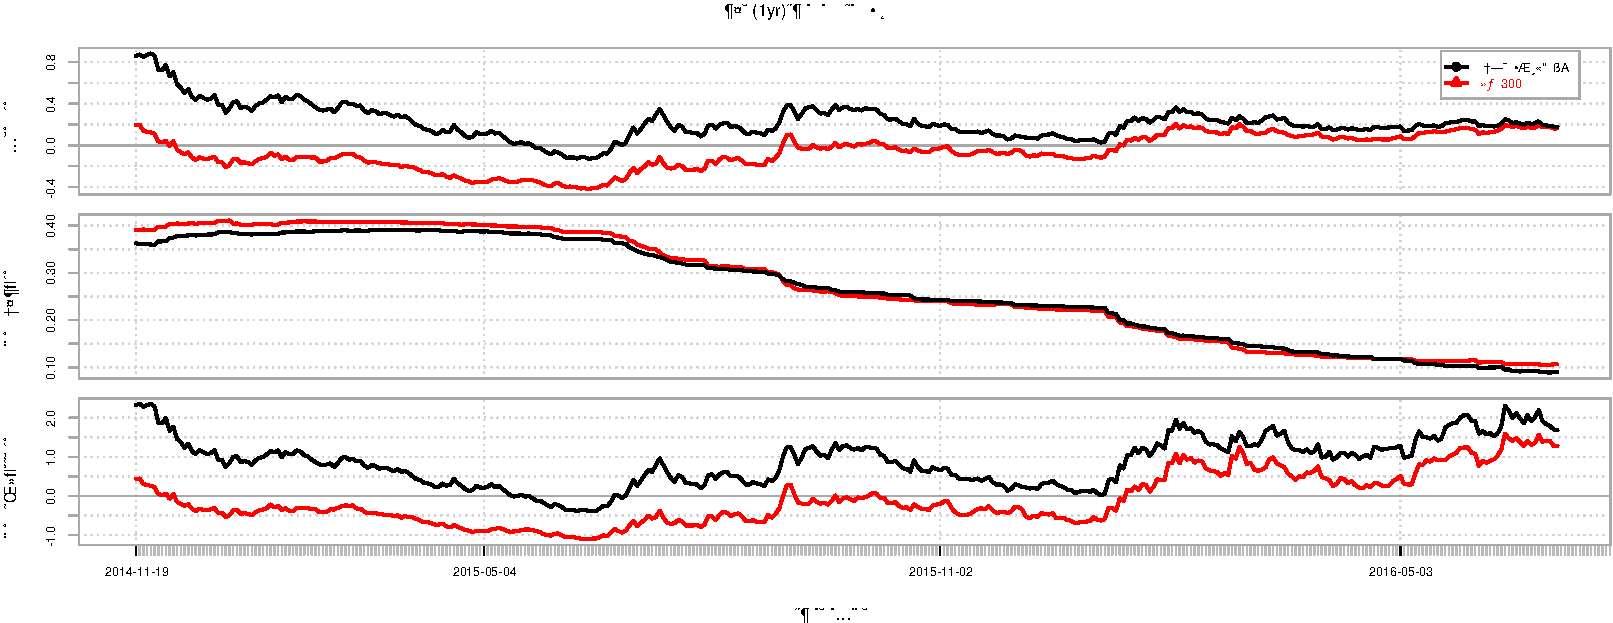
\includegraphics{linear_regression_files/figure-latex/unnamed-chunk-3-1.pdf}

首先是,这两组数据本就不太支持我们的模型。其次,模型描述的发生概率,不是因变量自身。

一个可能的改进是把线性函数\((-\infty,+\infty)\)的取值空间映射到概率空间\([0,1]\)上。这样做,只需要寻找一个满足一定性质的函数就可以,具体来说:

\begin{enumerate}
\def\labelenumi{\arabic{enumi}.}
\tightlist
\item
  光滑
\item
  单调
\end{enumerate}

这是两个比较好的性质。合在一起可以保证函数的逆函数也很漂亮,这是重要的。

比如: \[
h_i = \alpha + \beta x_i \\
g(p_i)=h_i
\]
其中\(g(\cdot)\)称为连接函数------将因变量与线性模型的输出连接起来的函数------可能的表达式为:
\[
h_i=g(p_i)=\log(\frac{p_i}{1-p_i})
\] 该函数的逆函数为: \[
p_i = \frac{1}{1+e^{-h_i}}
\]
我们依旧可以使用最大似然估计来建立这个回归模型。以下的R代码使用了glm函数来实现这一过程。

\begin{Shaded}
\begin{Highlighting}[]
\NormalTok{ber.logit<-}\KeywordTok{glm}\NormalTok{(y~x,}\DataTypeTok{family=}\KeywordTok{binomial}\NormalTok{())}
\KeywordTok{summary}\NormalTok{(ber.logit)}
\end{Highlighting}
\end{Shaded}

\begin{verbatim}
## 
## Call:
## glm(formula = y ~ x, family = binomial())
## 
## Deviance Residuals: 
##    Min      1Q  Median      3Q     Max  
## -1.623  -1.240   0.961   1.116   1.365  
## 
## Coefficients:
##             Estimate Std. Error z value Pr(>|z|)  
## (Intercept)   0.1456     0.1254   1.161   0.2458  
## x             3.8546     1.8220   2.116   0.0344 *
## ---
## Signif. codes:  0 '***' 0.001 '**' 0.01 '*' 0.05 '.' 0.1 ' ' 1
## 
## (Dispersion parameter for binomial family taken to be 1)
## 
##     Null deviance: 360.13  on 260  degrees of freedom
## Residual deviance: 354.79  on 259  degrees of freedom
## AIC: 358.79
## 
## Number of Fisher Scoring iterations: 3
\end{verbatim}

这样的连接函数多种多样,除了已经见到的(称为logit函数),我们还有逆正太累计分布函数,又称为probit函数。

\begin{Shaded}
\begin{Highlighting}[]
\NormalTok{ber.probit<-}\KeywordTok{glm}\NormalTok{(y~x,}\DataTypeTok{family=}\KeywordTok{binomial}\NormalTok{(}\DataTypeTok{link=}\StringTok{'probit'}\NormalTok{))}
\KeywordTok{summary}\NormalTok{(ber.probit)}
\end{Highlighting}
\end{Shaded}

\begin{verbatim}
## 
## Call:
## glm(formula = y ~ x, family = binomial(link = "probit"))
## 
## Deviance Residuals: 
##     Min       1Q   Median       3Q      Max  
## -1.6303  -1.2393   0.9606   1.1167   1.3662  
## 
## Coefficients:
##             Estimate Std. Error z value Pr(>|z|)  
## (Intercept)  0.09049    0.07828   1.156   0.2477  
## x            2.41217    1.08673   2.220   0.0264 *
## ---
## Signif. codes:  0 '***' 0.001 '**' 0.01 '*' 0.05 '.' 0.1 ' ' 1
## 
## (Dispersion parameter for binomial family taken to be 1)
## 
##     Null deviance: 360.13  on 260  degrees of freedom
## Residual deviance: 354.71  on 259  degrees of freedom
## AIC: 358.71
## 
## Number of Fisher Scoring iterations: 4
\end{verbatim}

我们总的来比较一下三个模型的结果

\begin{Shaded}
\begin{Highlighting}[]
\KeywordTok{plot}\NormalTok{(x,y)}
\KeywordTok{curve}\NormalTok{(}\KeywordTok{predict}\NormalTok{(ber, }\KeywordTok{data.frame}\NormalTok{(}\DataTypeTok{x =} \NormalTok{x)),}\DataTypeTok{add=}\OtherTok{TRUE}\NormalTok{,}\DataTypeTok{lty=}\DecValTok{1}\NormalTok{)}
\KeywordTok{curve}\NormalTok{(}\KeywordTok{predict}\NormalTok{(ber.logit, }\KeywordTok{data.frame}\NormalTok{(}\DataTypeTok{x =} \NormalTok{x), }\DataTypeTok{type =} \StringTok{"response"}\NormalTok{),}\DataTypeTok{add=}\OtherTok{TRUE}\NormalTok{,}\DataTypeTok{lty=}\DecValTok{2}\NormalTok{)}
\KeywordTok{curve}\NormalTok{(}\KeywordTok{predict}\NormalTok{(ber.probit, }\KeywordTok{data.frame}\NormalTok{(}\DataTypeTok{x =} \NormalTok{x), }\DataTypeTok{type =} \StringTok{"response"}\NormalTok{),}\DataTypeTok{add=}\OtherTok{TRUE}\NormalTok{,}\DataTypeTok{lty=}\DecValTok{3}\NormalTok{)}
\end{Highlighting}
\end{Shaded}

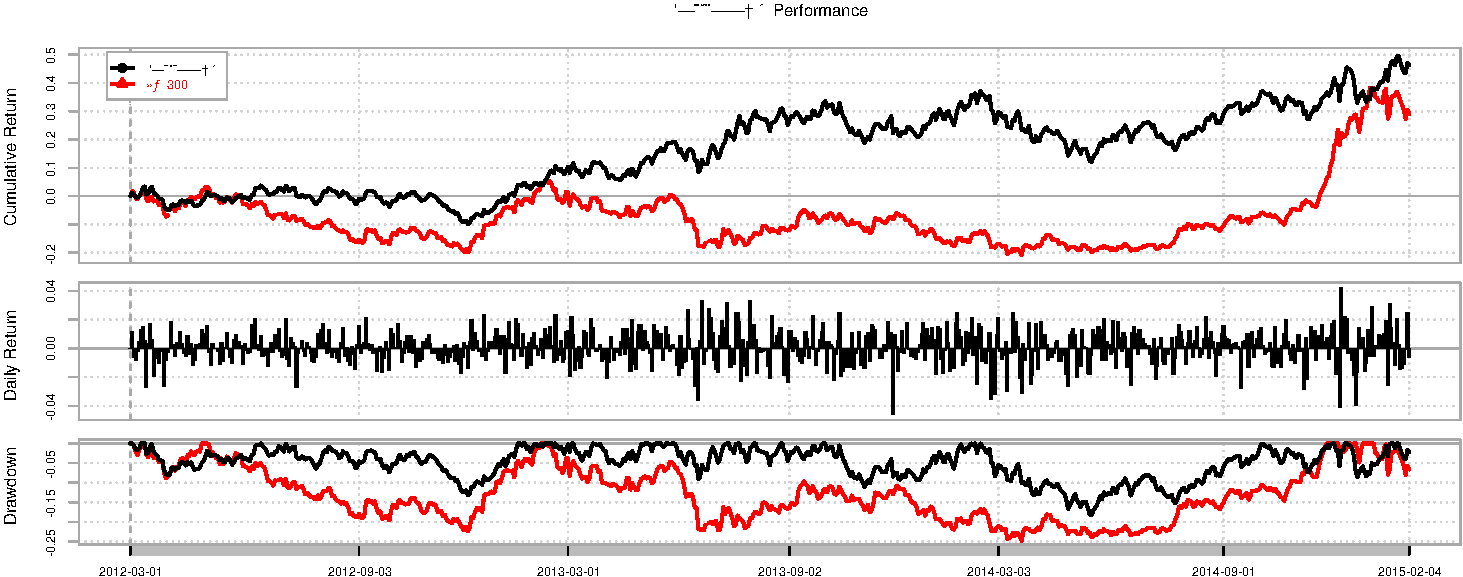
\includegraphics{linear_regression_files/figure-latex/unnamed-chunk-6-1.pdf}

\subsection{动态线性模型}

通常动态线性模型包括4个重要的可变参数\(\{F_t,G_t,V_t,W_t\}\):

\begin{itemize}
\tightlist
\item
  观测约束: \(Y_t = F_t \theta_t + v_t\),其中\(v_t \sim N(0,V_t)\)
\item
  系统约束:
  \(\theta_t = G_t \theta_{t-1} + \omega_t\),其中\(\omega_t\sim N(0,W_t)\)
\item
  先验概率: \(\theta_0\sim N(m_0,C_0)\)
\end{itemize}

其中,误差序列\(v_t\)与系统游动序列\(\omega_t\)是相互独立的,其各自也是独立的随机序列。系统如果存在任何的自相关性,都应该被\(F_t\)与\(G_t\)所蕴含的线性关系表达。当\(G_t=G\)时,系统约束显示出了了``差分不变''+随机噪声的特性,是介于简单线性模型和复杂线性模型之间的桥梁,往往成为我们有力的工具之一。

在文件pmi.csv中记录了中国自2008年以来每月报告的采购经理人指数,数据来自于中国物流与采购联合会网站。对于该数据的分析以及预测,使用一个模型参数为\(\{1,1,V,W_t \}\)的动态线性模型是可以的。数学上,

\begin{itemize}
\tightlist
\item
  观测约束:\(PMI_t = \theta_t + v_t\),其中\(v_t\sim N(0,V_t)\)
\item
  系统约束:\(\theta_t = \theta_{t-1} + w\),其中\(w\sim N(0,W)\)
\end{itemize}

可见\(\theta_t\)实际是PMI指数在t时刻的均值,在短期内我们认为该均值近似不变的,而长期则没有明确方向性的预测。因此,我们使用了一个随机游走过程来对\(\theta_t\)进行建模。当然不同的时期PMI的波动性不一样,这可能更多的来自于受调查对象的主观情绪,所以我们保持了\(V_t\)的时变性。

\begin{Shaded}
\begin{Highlighting}[]
\KeywordTok{library}\NormalTok{(purrr)}
\end{Highlighting}
\end{Shaded}

\begin{verbatim}
## 
## Attaching package: 'purrr'
\end{verbatim}

\begin{verbatim}
## The following objects are masked from 'package:foreach':
## 
##     accumulate, when
\end{verbatim}

\begin{verbatim}
## The following object is masked from 'package:plyr':
## 
##     compact
\end{verbatim}

\begin{verbatim}
## The following object is masked from 'package:scales':
## 
##     discard
\end{verbatim}

\begin{Shaded}
\begin{Highlighting}[]
\KeywordTok{library}\NormalTok{(dplyr)}
\end{Highlighting}
\end{Shaded}

\begin{verbatim}
## 
## Attaching package: 'dplyr'
\end{verbatim}

\begin{verbatim}
## The following objects are masked from 'package:plyr':
## 
##     arrange, count, desc, failwith, id, mutate, rename, summarise,
##     summarize
\end{verbatim}

\begin{verbatim}
## The following object is masked from 'package:nlme':
## 
##     collapse
\end{verbatim}

\begin{verbatim}
## The following objects are masked from 'package:lubridate':
## 
##     intersect, setdiff, union
\end{verbatim}

\begin{verbatim}
## The following objects are masked from 'package:xts':
## 
##     first, last
\end{verbatim}

\begin{verbatim}
## The following objects are masked from 'package:stats':
## 
##     filter, lag
\end{verbatim}

\begin{verbatim}
## The following objects are masked from 'package:base':
## 
##     intersect, setdiff, setequal, union
\end{verbatim}

\begin{Shaded}
\begin{Highlighting}[]
\NormalTok{p=}\KeywordTok{read.csv}\NormalTok{(}\StringTok{'./data/pmi.csv'}\NormalTok{,}\DataTypeTok{header=}\OtherTok{FALSE}\NormalTok{)}
\NormalTok{ad.year<-function(x)\{}\KeywordTok{as.yearmon}\NormalTok{(}\KeywordTok{paste}\NormalTok{(}\KeywordTok{substr}\NormalTok{(}\KeywordTok{as.character}\NormalTok{(x),}\DecValTok{1}\NormalTok{,}\DecValTok{4}\NormalTok{),}\KeywordTok{substr}\NormalTok{(}\KeywordTok{as.character}\NormalTok{(x),}\DecValTok{6}\NormalTok{,}\DecValTok{7}\NormalTok{),}\DataTypeTok{sep=}\StringTok{'-'}\NormalTok{))\}}
\NormalTok{p$V1<-}\KeywordTok{unlist}\NormalTok{(p$V1 %>%}\StringTok{ }\KeywordTok{map}\NormalTok{(ad.year))}
\NormalTok{p=}\KeywordTok{arrange}\NormalTok{(p,V1)}
\NormalTok{myPMI<-function(b)}
\NormalTok{\{}
  \NormalTok{m<-}\KeywordTok{dlmModReg}\NormalTok{(p$V2,}\OtherTok{FALSE}\NormalTok{,}\DataTypeTok{dW=}\NormalTok{b[}\DecValTok{1}\NormalTok{]^}\DecValTok{2}\NormalTok{,}\DataTypeTok{m0=}\DecValTok{50}\NormalTok{)}
  \NormalTok{m$JFF<-}\KeywordTok{matrix}\NormalTok{(}\DecValTok{0}\NormalTok{,}\DataTypeTok{nr=}\DecValTok{1}\NormalTok{,}\DataTypeTok{nc=}\DecValTok{1}\NormalTok{)}
  \KeywordTok{return}\NormalTok{(m)}
\NormalTok{\}}
\NormalTok{fit<-}\KeywordTok{dlmMLE}\NormalTok{(p$V2,}\DataTypeTok{parm=}\FloatTok{0.1}\NormalTok{,}\DataTypeTok{build=}\NormalTok{myPMI)}
\NormalTok{mod<-}\KeywordTok{myPMI}\NormalTok{(fit$par)}
\NormalTok{filted<-}\KeywordTok{dlmFilter}\NormalTok{(p$V2,mod)}
\KeywordTok{plot}\NormalTok{(}\KeywordTok{cbind}\NormalTok{(p$V1,filted$m[-}\DecValTok{1}\NormalTok{]),}\DataTypeTok{col=}\KeywordTok{c}\NormalTok{(}\StringTok{'black'}\NormalTok{,}\StringTok{'red'}\NormalTok{),}\DataTypeTok{xlab=}\StringTok{'日期'}\NormalTok{,}\DataTypeTok{ylab=}\StringTok{'制造业PMI'}\NormalTok{)}
\end{Highlighting}
\end{Shaded}

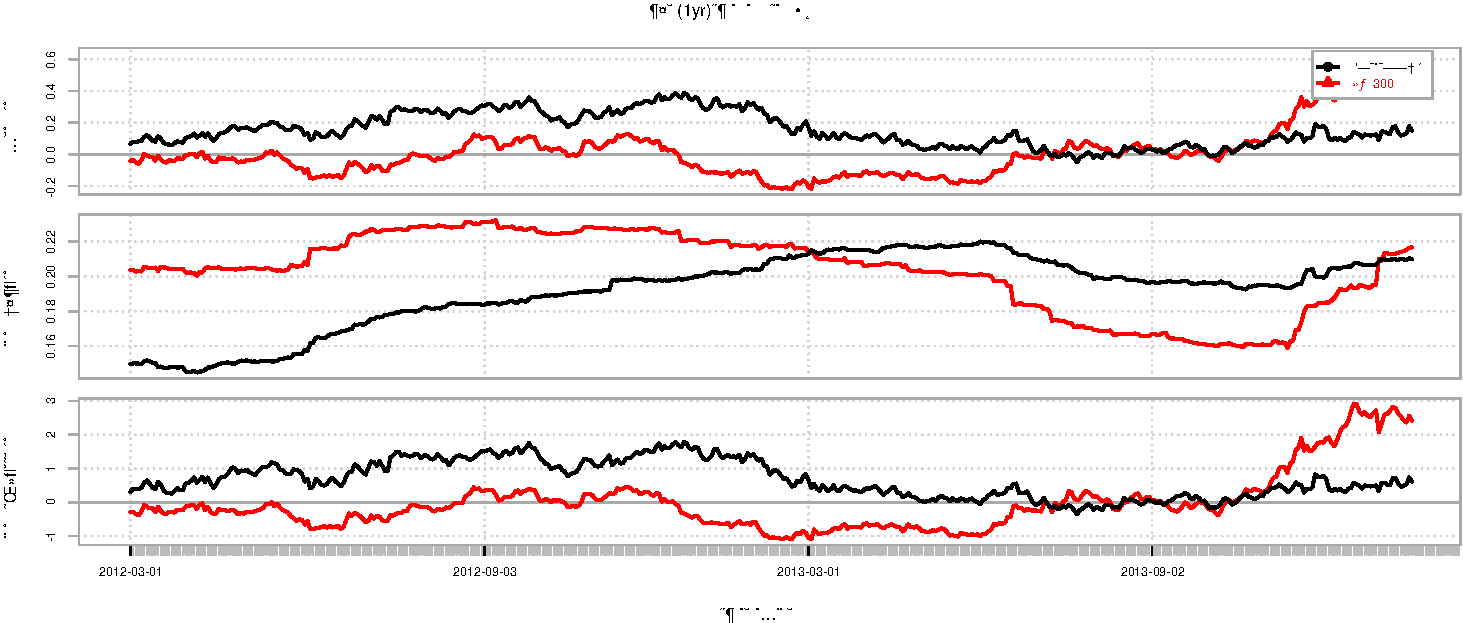
\includegraphics{linear_regression_files/figure-latex/unnamed-chunk-7-1.pdf}

这显然出现了过分拟合的情况,也就是对于PMI实际上不需要那么复杂的模型。模型的自由度太多,我们考虑降低维度,将\(V_t\)确定为\(V\)。

\begin{Shaded}
\begin{Highlighting}[]
\NormalTok{myPMI2<-function(b)}
\NormalTok{\{}
  \NormalTok{m<-}\KeywordTok{dlmModReg}\NormalTok{(p$V2,}\OtherTok{FALSE}\NormalTok{,}\DataTypeTok{dW=}\NormalTok{b[}\DecValTok{1}\NormalTok{]^}\DecValTok{2}\NormalTok{,}\DataTypeTok{dV=}\NormalTok{b[}\DecValTok{2}\NormalTok{]^}\DecValTok{2}\NormalTok{,}\DataTypeTok{m0=}\DecValTok{50}\NormalTok{)}
  \NormalTok{m$JFF<-}\KeywordTok{matrix}\NormalTok{(}\DecValTok{0}\NormalTok{,}\DataTypeTok{nr=}\DecValTok{1}\NormalTok{,}\DataTypeTok{nc=}\DecValTok{1}\NormalTok{)}
  \KeywordTok{return}\NormalTok{(m)}
\NormalTok{\}}
\NormalTok{fit<-}\KeywordTok{dlmMLE}\NormalTok{(p$V2,}\DataTypeTok{parm=}\KeywordTok{c}\NormalTok{(}\FloatTok{0.1}\NormalTok{,}\FloatTok{0.1}\NormalTok{),}\DataTypeTok{build=}\NormalTok{myPMI2)}
\NormalTok{mod<-}\KeywordTok{myPMI}\NormalTok{(fit$par)}
\NormalTok{filted<-}\KeywordTok{dlmFilter}\NormalTok{(p$V2,mod)}
\KeywordTok{plot}\NormalTok{(}\KeywordTok{cbind}\NormalTok{(p$V1,filted$m[-}\DecValTok{1}\NormalTok{]),}\DataTypeTok{col=}\KeywordTok{c}\NormalTok{(}\StringTok{'black'}\NormalTok{,}\StringTok{'red'}\NormalTok{),}\DataTypeTok{xlab=}\StringTok{'日期'}\NormalTok{,}\DataTypeTok{ylab=}\StringTok{'制造业PMI'}\NormalTok{)}
\end{Highlighting}
\end{Shaded}

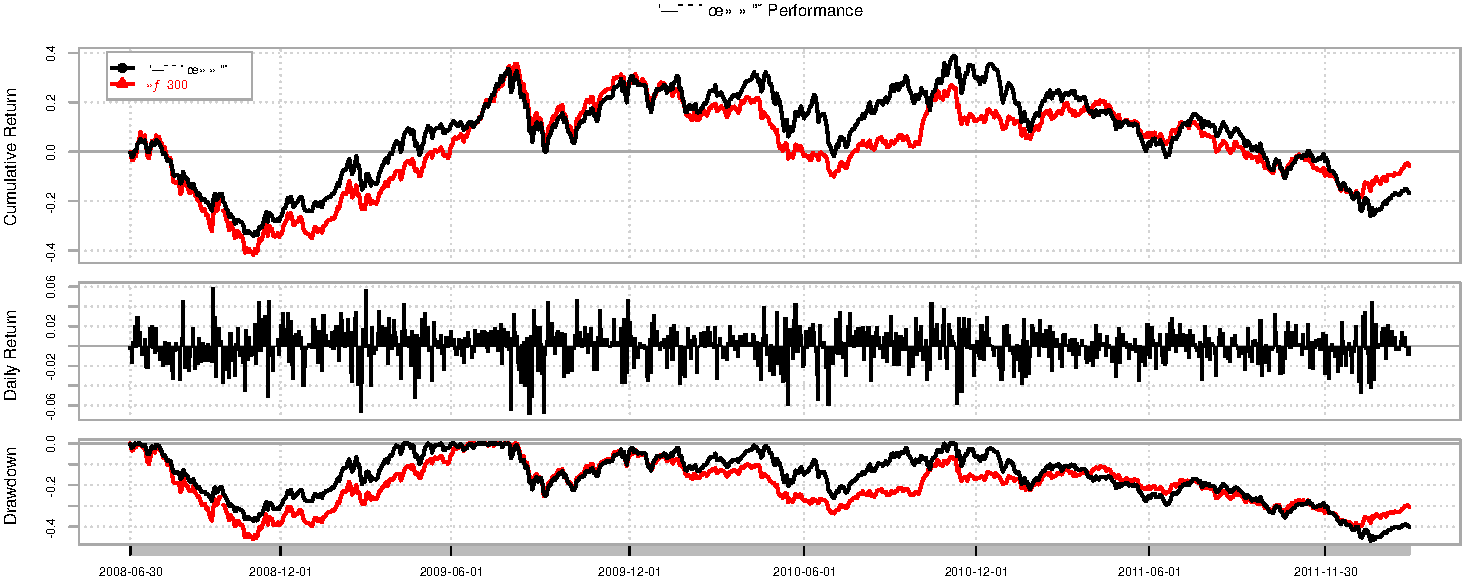
\includegraphics{linear_regression_files/figure-latex/unnamed-chunk-8-1.pdf}
总感觉使用动态线性模型用来拟合PMI的数据有过分拟合的嫌疑。
一般意义上,当观测量\(Y_t\)被如下表达的时候 \[
Y_t=\theta_t + v_t
\]
\(\theta_t\)是该序列在t时刻的水平级(level),\(v_t\)为观测误差。水平级(level)的时间变化,可以描述为
\[
\theta_t = \theta_{t-1}+\omega_t\ \ \ \ \ \omega_t\sim N(0,W_t)
\]
是一个随机走过程,\(\omega_t\)被成为系统演化噪声。这样的随机走过程描述的水平级(level)具备局部稳定性。这种类型的动态模型对于短期预测是有用的。因为它的预测函数\(f_t(\cdot)\)是一个衡量,表达如下
\[
f_t(k)=E(Y_{t+k}|D_t)=E(\theta_t|D_t)=m_t
\]
其中,\(D_t\)代表t时刻时存在的所有信息,\(m_t\)是\(\theta_t\)的后验的条件均值。也是因为这种局部稳定性,所以我们一般要求观测噪声\(V_t\)要显著的大于系统演化噪声\(W_t\)。

\begin{Shaded}
\begin{Highlighting}[]
\KeywordTok{require}\NormalTok{(dlm)}
\KeywordTok{require}\NormalTok{(reshape2)}
\end{Highlighting}
\end{Shaded}

\begin{verbatim}
## Loading required package: reshape2
\end{verbatim}

\begin{verbatim}
## 
## Attaching package: 'reshape2'
\end{verbatim}

\begin{verbatim}
## The following object is masked from 'package:tidyr':
## 
##     smiths
\end{verbatim}

\begin{Shaded}
\begin{Highlighting}[]
\KeywordTok{require}\NormalTok{(ggplot2)}
\end{Highlighting}
\end{Shaded}

\begin{verbatim}
## Loading required package: ggplot2
\end{verbatim}

\begin{verbatim}
## 
## Attaching package: 'ggplot2'
\end{verbatim}

\begin{verbatim}
## The following object is masked from 'package:dlm':
## 
##     %+%
\end{verbatim}

\begin{Shaded}
\begin{Highlighting}[]
\KeywordTok{set.seed}\NormalTok{(}\DecValTok{12345}\NormalTok{)}
\NormalTok{v=}\KeywordTok{rnorm}\NormalTok{(}\DecValTok{100}\NormalTok{)}
\NormalTok{w=}\FloatTok{0.05}\NormalTok{*}\KeywordTok{rnorm}\NormalTok{(}\DecValTok{100}\NormalTok{)}
\NormalTok{bigw=}\DecValTok{10}\NormalTok{*w}
\NormalTok{bigmu=}\KeywordTok{rep}\NormalTok{(}\DecValTok{0}\NormalTok{,}\DecValTok{100}\NormalTok{)}
\NormalTok{mu0=}\DecValTok{1}
\NormalTok{mu=}\KeywordTok{rep}\NormalTok{(}\DecValTok{0}\NormalTok{,}\DecValTok{100}\NormalTok{)}
\NormalTok{y=}\KeywordTok{rep}\NormalTok{(}\DecValTok{0}\NormalTok{,}\DecValTok{100}\NormalTok{)}
\NormalTok{bigy=}\KeywordTok{rep}\NormalTok{(}\DecValTok{0}\NormalTok{,}\DecValTok{100}\NormalTok{)}
\NormalTok{mu[}\DecValTok{1}\NormalTok{]=mu0}
\NormalTok{bigmu[}\DecValTok{1}\NormalTok{]=mu0}
\NormalTok{for(i in }\DecValTok{1}\NormalTok{:}\DecValTok{99}\NormalTok{)}
\NormalTok{\{}
  \NormalTok{mu[i]=mu[i]+w[i]}
  \NormalTok{bigmu[i]=bigmu[i]+bigw[i]}
  \NormalTok{y[i]=mu[i]+v[i]}
  \NormalTok{bigy[i]=bigmu[i]+v[i]}
  \NormalTok{mu[i}\DecValTok{+1}\NormalTok{]=mu[i]}
  \NormalTok{bigmu[i}\DecValTok{+1}\NormalTok{]=bigmu[i]}
\NormalTok{\}}
\NormalTok{mu[}\DecValTok{100}\NormalTok{]=mu[}\DecValTok{100}\NormalTok{]+w[}\DecValTok{100}\NormalTok{]}
\NormalTok{bigmu[}\DecValTok{100}\NormalTok{]=bigmu[}\DecValTok{100}\NormalTok{]+bigw[}\DecValTok{100}\NormalTok{]}
\NormalTok{y[}\DecValTok{100}\NormalTok{]=mu[}\DecValTok{100}\NormalTok{]+v[}\DecValTok{100}\NormalTok{]}
\NormalTok{bigy[}\DecValTok{100}\NormalTok{]=bigmu[}\DecValTok{100}\NormalTok{]+v[}\DecValTok{100}\NormalTok{]}
\NormalTok{data=}\KeywordTok{data.frame}\NormalTok{(}\DataTypeTok{level=}\NormalTok{mu,}\DataTypeTok{data=}\NormalTok{y)}
\NormalTok{data$date=}\KeywordTok{seq}\NormalTok{(}\KeywordTok{as.Date}\NormalTok{(}\StringTok{'2010-01-01'}\NormalTok{),}\DataTypeTok{by=}\StringTok{'day'}\NormalTok{,}\DataTypeTok{length.out=}\DecValTok{100}\NormalTok{)}
\NormalTok{d=}\KeywordTok{melt}\NormalTok{(data,}\DataTypeTok{id.vars=}\StringTok{'date'}\NormalTok{)}
\KeywordTok{ggplot}\NormalTok{(d,}\KeywordTok{aes}\NormalTok{(}\DataTypeTok{x=}\NormalTok{date,}\DataTypeTok{y=}\NormalTok{value,}\DataTypeTok{colour=}\NormalTok{variable,}\DataTypeTok{group=}\NormalTok{variable))+}\KeywordTok{geom_line}\NormalTok{()+}\KeywordTok{ggtitle}\NormalTok{(}\StringTok{'Simulated GLM with W/V=0.05'}\NormalTok{)}
\end{Highlighting}
\end{Shaded}

\begin{verbatim}
## Warning in grid.Call(C_textBounds, as.graphicsAnnot(x$label), x$x, x$y, :
## conversion failure on '1月' in 'mbcsToSbcs': dot substituted for <e6>
\end{verbatim}

\begin{verbatim}
## Warning in grid.Call(C_textBounds, as.graphicsAnnot(x$label), x$x, x$y, :
## conversion failure on '1月' in 'mbcsToSbcs': dot substituted for <9c>
\end{verbatim}

\begin{verbatim}
## Warning in grid.Call(C_textBounds, as.graphicsAnnot(x$label), x$x, x$y, :
## conversion failure on '1月' in 'mbcsToSbcs': dot substituted for <88>
\end{verbatim}

\begin{verbatim}
## Warning in grid.Call(C_textBounds, as.graphicsAnnot(x$label), x$x, x$y, :
## conversion failure on '2月' in 'mbcsToSbcs': dot substituted for <e6>
\end{verbatim}

\begin{verbatim}
## Warning in grid.Call(C_textBounds, as.graphicsAnnot(x$label), x$x, x$y, :
## conversion failure on '2月' in 'mbcsToSbcs': dot substituted for <9c>
\end{verbatim}

\begin{verbatim}
## Warning in grid.Call(C_textBounds, as.graphicsAnnot(x$label), x$x, x$y, :
## conversion failure on '2月' in 'mbcsToSbcs': dot substituted for <88>
\end{verbatim}

\begin{verbatim}
## Warning in grid.Call(C_textBounds, as.graphicsAnnot(x$label), x$x, x$y, :
## conversion failure on '3月' in 'mbcsToSbcs': dot substituted for <e6>
\end{verbatim}

\begin{verbatim}
## Warning in grid.Call(C_textBounds, as.graphicsAnnot(x$label), x$x, x$y, :
## conversion failure on '3月' in 'mbcsToSbcs': dot substituted for <9c>
\end{verbatim}

\begin{verbatim}
## Warning in grid.Call(C_textBounds, as.graphicsAnnot(x$label), x$x, x$y, :
## conversion failure on '3月' in 'mbcsToSbcs': dot substituted for <88>
\end{verbatim}

\begin{verbatim}
## Warning in grid.Call(C_textBounds, as.graphicsAnnot(x$label), x$x, x$y, :
## conversion failure on '4月' in 'mbcsToSbcs': dot substituted for <e6>
\end{verbatim}

\begin{verbatim}
## Warning in grid.Call(C_textBounds, as.graphicsAnnot(x$label), x$x, x$y, :
## conversion failure on '4月' in 'mbcsToSbcs': dot substituted for <9c>
\end{verbatim}

\begin{verbatim}
## Warning in grid.Call(C_textBounds, as.graphicsAnnot(x$label), x$x, x$y, :
## conversion failure on '4月' in 'mbcsToSbcs': dot substituted for <88>
\end{verbatim}

\begin{verbatim}
## Warning in grid.Call(C_textBounds, as.graphicsAnnot(x$label), x$x, x$y, :
## conversion failure on '1月' in 'mbcsToSbcs': dot substituted for <e6>
\end{verbatim}

\begin{verbatim}
## Warning in grid.Call(C_textBounds, as.graphicsAnnot(x$label), x$x, x$y, :
## conversion failure on '1月' in 'mbcsToSbcs': dot substituted for <9c>
\end{verbatim}

\begin{verbatim}
## Warning in grid.Call(C_textBounds, as.graphicsAnnot(x$label), x$x, x$y, :
## conversion failure on '1月' in 'mbcsToSbcs': dot substituted for <88>
\end{verbatim}

\begin{verbatim}
## Warning in grid.Call(C_textBounds, as.graphicsAnnot(x$label), x$x, x$y, :
## conversion failure on '2月' in 'mbcsToSbcs': dot substituted for <e6>
\end{verbatim}

\begin{verbatim}
## Warning in grid.Call(C_textBounds, as.graphicsAnnot(x$label), x$x, x$y, :
## conversion failure on '2月' in 'mbcsToSbcs': dot substituted for <9c>
\end{verbatim}

\begin{verbatim}
## Warning in grid.Call(C_textBounds, as.graphicsAnnot(x$label), x$x, x$y, :
## conversion failure on '2月' in 'mbcsToSbcs': dot substituted for <88>
\end{verbatim}

\begin{verbatim}
## Warning in grid.Call(C_textBounds, as.graphicsAnnot(x$label), x$x, x$y, :
## conversion failure on '3月' in 'mbcsToSbcs': dot substituted for <e6>
\end{verbatim}

\begin{verbatim}
## Warning in grid.Call(C_textBounds, as.graphicsAnnot(x$label), x$x, x$y, :
## conversion failure on '3月' in 'mbcsToSbcs': dot substituted for <9c>
\end{verbatim}

\begin{verbatim}
## Warning in grid.Call(C_textBounds, as.graphicsAnnot(x$label), x$x, x$y, :
## conversion failure on '3月' in 'mbcsToSbcs': dot substituted for <88>
\end{verbatim}

\begin{verbatim}
## Warning in grid.Call(C_textBounds, as.graphicsAnnot(x$label), x$x, x$y, :
## conversion failure on '4月' in 'mbcsToSbcs': dot substituted for <e6>
\end{verbatim}

\begin{verbatim}
## Warning in grid.Call(C_textBounds, as.graphicsAnnot(x$label), x$x, x$y, :
## conversion failure on '4月' in 'mbcsToSbcs': dot substituted for <9c>
\end{verbatim}

\begin{verbatim}
## Warning in grid.Call(C_textBounds, as.graphicsAnnot(x$label), x$x, x$y, :
## conversion failure on '4月' in 'mbcsToSbcs': dot substituted for <88>
\end{verbatim}

\begin{verbatim}
## Warning in grid.Call(C_textBounds, as.graphicsAnnot(x$label), x$x, x$y, :
## conversion failure on '1月' in 'mbcsToSbcs': dot substituted for <e6>
\end{verbatim}

\begin{verbatim}
## Warning in grid.Call(C_textBounds, as.graphicsAnnot(x$label), x$x, x$y, :
## conversion failure on '1月' in 'mbcsToSbcs': dot substituted for <9c>
\end{verbatim}

\begin{verbatim}
## Warning in grid.Call(C_textBounds, as.graphicsAnnot(x$label), x$x, x$y, :
## conversion failure on '1月' in 'mbcsToSbcs': dot substituted for <88>
\end{verbatim}

\begin{verbatim}
## Warning in grid.Call(C_textBounds, as.graphicsAnnot(x$label), x$x, x$y, :
## conversion failure on '2月' in 'mbcsToSbcs': dot substituted for <e6>
\end{verbatim}

\begin{verbatim}
## Warning in grid.Call(C_textBounds, as.graphicsAnnot(x$label), x$x, x$y, :
## conversion failure on '2月' in 'mbcsToSbcs': dot substituted for <9c>
\end{verbatim}

\begin{verbatim}
## Warning in grid.Call(C_textBounds, as.graphicsAnnot(x$label), x$x, x$y, :
## conversion failure on '2月' in 'mbcsToSbcs': dot substituted for <88>
\end{verbatim}

\begin{verbatim}
## Warning in grid.Call(C_textBounds, as.graphicsAnnot(x$label), x$x, x$y, :
## conversion failure on '3月' in 'mbcsToSbcs': dot substituted for <e6>
\end{verbatim}

\begin{verbatim}
## Warning in grid.Call(C_textBounds, as.graphicsAnnot(x$label), x$x, x$y, :
## conversion failure on '3月' in 'mbcsToSbcs': dot substituted for <9c>
\end{verbatim}

\begin{verbatim}
## Warning in grid.Call(C_textBounds, as.graphicsAnnot(x$label), x$x, x$y, :
## conversion failure on '3月' in 'mbcsToSbcs': dot substituted for <88>
\end{verbatim}

\begin{verbatim}
## Warning in grid.Call(C_textBounds, as.graphicsAnnot(x$label), x$x, x$y, :
## conversion failure on '4月' in 'mbcsToSbcs': dot substituted for <e6>
\end{verbatim}

\begin{verbatim}
## Warning in grid.Call(C_textBounds, as.graphicsAnnot(x$label), x$x, x$y, :
## conversion failure on '4月' in 'mbcsToSbcs': dot substituted for <9c>
\end{verbatim}

\begin{verbatim}
## Warning in grid.Call(C_textBounds, as.graphicsAnnot(x$label), x$x, x$y, :
## conversion failure on '4月' in 'mbcsToSbcs': dot substituted for <88>
\end{verbatim}

\begin{verbatim}
## Warning in grid.Call(C_textBounds, as.graphicsAnnot(x$label), x$x, x$y, :
## conversion failure on '1月' in 'mbcsToSbcs': dot substituted for <e6>
\end{verbatim}

\begin{verbatim}
## Warning in grid.Call(C_textBounds, as.graphicsAnnot(x$label), x$x, x$y, :
## conversion failure on '1月' in 'mbcsToSbcs': dot substituted for <9c>
\end{verbatim}

\begin{verbatim}
## Warning in grid.Call(C_textBounds, as.graphicsAnnot(x$label), x$x, x$y, :
## conversion failure on '1月' in 'mbcsToSbcs': dot substituted for <88>
\end{verbatim}

\begin{verbatim}
## Warning in grid.Call(C_textBounds, as.graphicsAnnot(x$label), x$x, x$y, :
## conversion failure on '2月' in 'mbcsToSbcs': dot substituted for <e6>
\end{verbatim}

\begin{verbatim}
## Warning in grid.Call(C_textBounds, as.graphicsAnnot(x$label), x$x, x$y, :
## conversion failure on '2月' in 'mbcsToSbcs': dot substituted for <9c>
\end{verbatim}

\begin{verbatim}
## Warning in grid.Call(C_textBounds, as.graphicsAnnot(x$label), x$x, x$y, :
## conversion failure on '2月' in 'mbcsToSbcs': dot substituted for <88>
\end{verbatim}

\begin{verbatim}
## Warning in grid.Call(C_textBounds, as.graphicsAnnot(x$label), x$x, x$y, :
## conversion failure on '3月' in 'mbcsToSbcs': dot substituted for <e6>
\end{verbatim}

\begin{verbatim}
## Warning in grid.Call(C_textBounds, as.graphicsAnnot(x$label), x$x, x$y, :
## conversion failure on '3月' in 'mbcsToSbcs': dot substituted for <9c>
\end{verbatim}

\begin{verbatim}
## Warning in grid.Call(C_textBounds, as.graphicsAnnot(x$label), x$x, x$y, :
## conversion failure on '3月' in 'mbcsToSbcs': dot substituted for <88>
\end{verbatim}

\begin{verbatim}
## Warning in grid.Call(C_textBounds, as.graphicsAnnot(x$label), x$x, x$y, :
## conversion failure on '4月' in 'mbcsToSbcs': dot substituted for <e6>
\end{verbatim}

\begin{verbatim}
## Warning in grid.Call(C_textBounds, as.graphicsAnnot(x$label), x$x, x$y, :
## conversion failure on '4月' in 'mbcsToSbcs': dot substituted for <9c>
\end{verbatim}

\begin{verbatim}
## Warning in grid.Call(C_textBounds, as.graphicsAnnot(x$label), x$x, x$y, :
## conversion failure on '4月' in 'mbcsToSbcs': dot substituted for <88>
\end{verbatim}

\begin{verbatim}
## Warning in grid.Call(C_textBounds, as.graphicsAnnot(x$label), x$x, x$y, :
## conversion failure on '1月' in 'mbcsToSbcs': dot substituted for <e6>
\end{verbatim}

\begin{verbatim}
## Warning in grid.Call(C_textBounds, as.graphicsAnnot(x$label), x$x, x$y, :
## conversion failure on '1月' in 'mbcsToSbcs': dot substituted for <9c>
\end{verbatim}

\begin{verbatim}
## Warning in grid.Call(C_textBounds, as.graphicsAnnot(x$label), x$x, x$y, :
## conversion failure on '1月' in 'mbcsToSbcs': dot substituted for <88>
\end{verbatim}

\begin{verbatim}
## Warning in grid.Call(C_textBounds, as.graphicsAnnot(x$label), x$x, x$y, :
## conversion failure on '2月' in 'mbcsToSbcs': dot substituted for <e6>
\end{verbatim}

\begin{verbatim}
## Warning in grid.Call(C_textBounds, as.graphicsAnnot(x$label), x$x, x$y, :
## conversion failure on '2月' in 'mbcsToSbcs': dot substituted for <9c>
\end{verbatim}

\begin{verbatim}
## Warning in grid.Call(C_textBounds, as.graphicsAnnot(x$label), x$x, x$y, :
## conversion failure on '2月' in 'mbcsToSbcs': dot substituted for <88>
\end{verbatim}

\begin{verbatim}
## Warning in grid.Call(C_textBounds, as.graphicsAnnot(x$label), x$x, x$y, :
## conversion failure on '3月' in 'mbcsToSbcs': dot substituted for <e6>
\end{verbatim}

\begin{verbatim}
## Warning in grid.Call(C_textBounds, as.graphicsAnnot(x$label), x$x, x$y, :
## conversion failure on '3月' in 'mbcsToSbcs': dot substituted for <9c>
\end{verbatim}

\begin{verbatim}
## Warning in grid.Call(C_textBounds, as.graphicsAnnot(x$label), x$x, x$y, :
## conversion failure on '3月' in 'mbcsToSbcs': dot substituted for <88>
\end{verbatim}

\begin{verbatim}
## Warning in grid.Call(C_textBounds, as.graphicsAnnot(x$label), x$x, x$y, :
## conversion failure on '4月' in 'mbcsToSbcs': dot substituted for <e6>
\end{verbatim}

\begin{verbatim}
## Warning in grid.Call(C_textBounds, as.graphicsAnnot(x$label), x$x, x$y, :
## conversion failure on '4月' in 'mbcsToSbcs': dot substituted for <9c>
\end{verbatim}

\begin{verbatim}
## Warning in grid.Call(C_textBounds, as.graphicsAnnot(x$label), x$x, x$y, :
## conversion failure on '4月' in 'mbcsToSbcs': dot substituted for <88>
\end{verbatim}

\begin{verbatim}
## Warning in grid.Call(C_textBounds, as.graphicsAnnot(x$label), x$x, x$y, :
## conversion failure on '1月' in 'mbcsToSbcs': dot substituted for <e6>
\end{verbatim}

\begin{verbatim}
## Warning in grid.Call(C_textBounds, as.graphicsAnnot(x$label), x$x, x$y, :
## conversion failure on '1月' in 'mbcsToSbcs': dot substituted for <9c>
\end{verbatim}

\begin{verbatim}
## Warning in grid.Call(C_textBounds, as.graphicsAnnot(x$label), x$x, x$y, :
## conversion failure on '1月' in 'mbcsToSbcs': dot substituted for <88>
\end{verbatim}

\begin{verbatim}
## Warning in grid.Call(C_textBounds, as.graphicsAnnot(x$label), x$x, x$y, :
## conversion failure on '2月' in 'mbcsToSbcs': dot substituted for <e6>
\end{verbatim}

\begin{verbatim}
## Warning in grid.Call(C_textBounds, as.graphicsAnnot(x$label), x$x, x$y, :
## conversion failure on '2月' in 'mbcsToSbcs': dot substituted for <9c>
\end{verbatim}

\begin{verbatim}
## Warning in grid.Call(C_textBounds, as.graphicsAnnot(x$label), x$x, x$y, :
## conversion failure on '2月' in 'mbcsToSbcs': dot substituted for <88>
\end{verbatim}

\begin{verbatim}
## Warning in grid.Call(C_textBounds, as.graphicsAnnot(x$label), x$x, x$y, :
## conversion failure on '3月' in 'mbcsToSbcs': dot substituted for <e6>
\end{verbatim}

\begin{verbatim}
## Warning in grid.Call(C_textBounds, as.graphicsAnnot(x$label), x$x, x$y, :
## conversion failure on '3月' in 'mbcsToSbcs': dot substituted for <9c>
\end{verbatim}

\begin{verbatim}
## Warning in grid.Call(C_textBounds, as.graphicsAnnot(x$label), x$x, x$y, :
## conversion failure on '3月' in 'mbcsToSbcs': dot substituted for <88>
\end{verbatim}

\begin{verbatim}
## Warning in grid.Call(C_textBounds, as.graphicsAnnot(x$label), x$x, x$y, :
## conversion failure on '4月' in 'mbcsToSbcs': dot substituted for <e6>
\end{verbatim}

\begin{verbatim}
## Warning in grid.Call(C_textBounds, as.graphicsAnnot(x$label), x$x, x$y, :
## conversion failure on '4月' in 'mbcsToSbcs': dot substituted for <9c>
\end{verbatim}

\begin{verbatim}
## Warning in grid.Call(C_textBounds, as.graphicsAnnot(x$label), x$x, x$y, :
## conversion failure on '4月' in 'mbcsToSbcs': dot substituted for <88>
\end{verbatim}

\begin{verbatim}
## Warning in grid.Call(C_textBounds, as.graphicsAnnot(x$label), x$x, x$y, :
## conversion failure on '1月' in 'mbcsToSbcs': dot substituted for <e6>
\end{verbatim}

\begin{verbatim}
## Warning in grid.Call(C_textBounds, as.graphicsAnnot(x$label), x$x, x$y, :
## conversion failure on '1月' in 'mbcsToSbcs': dot substituted for <9c>
\end{verbatim}

\begin{verbatim}
## Warning in grid.Call(C_textBounds, as.graphicsAnnot(x$label), x$x, x$y, :
## conversion failure on '1月' in 'mbcsToSbcs': dot substituted for <88>
\end{verbatim}

\begin{verbatim}
## Warning in grid.Call(C_textBounds, as.graphicsAnnot(x$label), x$x, x$y, :
## conversion failure on '2月' in 'mbcsToSbcs': dot substituted for <e6>
\end{verbatim}

\begin{verbatim}
## Warning in grid.Call(C_textBounds, as.graphicsAnnot(x$label), x$x, x$y, :
## conversion failure on '2月' in 'mbcsToSbcs': dot substituted for <9c>
\end{verbatim}

\begin{verbatim}
## Warning in grid.Call(C_textBounds, as.graphicsAnnot(x$label), x$x, x$y, :
## conversion failure on '2月' in 'mbcsToSbcs': dot substituted for <88>
\end{verbatim}

\begin{verbatim}
## Warning in grid.Call(C_textBounds, as.graphicsAnnot(x$label), x$x, x$y, :
## conversion failure on '3月' in 'mbcsToSbcs': dot substituted for <e6>
\end{verbatim}

\begin{verbatim}
## Warning in grid.Call(C_textBounds, as.graphicsAnnot(x$label), x$x, x$y, :
## conversion failure on '3月' in 'mbcsToSbcs': dot substituted for <9c>
\end{verbatim}

\begin{verbatim}
## Warning in grid.Call(C_textBounds, as.graphicsAnnot(x$label), x$x, x$y, :
## conversion failure on '3月' in 'mbcsToSbcs': dot substituted for <88>
\end{verbatim}

\begin{verbatim}
## Warning in grid.Call(C_textBounds, as.graphicsAnnot(x$label), x$x, x$y, :
## conversion failure on '4月' in 'mbcsToSbcs': dot substituted for <e6>
\end{verbatim}

\begin{verbatim}
## Warning in grid.Call(C_textBounds, as.graphicsAnnot(x$label), x$x, x$y, :
## conversion failure on '4月' in 'mbcsToSbcs': dot substituted for <9c>
\end{verbatim}

\begin{verbatim}
## Warning in grid.Call(C_textBounds, as.graphicsAnnot(x$label), x$x, x$y, :
## conversion failure on '4月' in 'mbcsToSbcs': dot substituted for <88>
\end{verbatim}

\begin{verbatim}
## Warning in grid.Call(C_textBounds, as.graphicsAnnot(x$label), x$x, x$y, :
## conversion failure on '1月' in 'mbcsToSbcs': dot substituted for <e6>
\end{verbatim}

\begin{verbatim}
## Warning in grid.Call(C_textBounds, as.graphicsAnnot(x$label), x$x, x$y, :
## conversion failure on '1月' in 'mbcsToSbcs': dot substituted for <9c>
\end{verbatim}

\begin{verbatim}
## Warning in grid.Call(C_textBounds, as.graphicsAnnot(x$label), x$x, x$y, :
## conversion failure on '1月' in 'mbcsToSbcs': dot substituted for <88>
\end{verbatim}

\begin{verbatim}
## Warning in grid.Call(C_textBounds, as.graphicsAnnot(x$label), x$x, x$y, :
## conversion failure on '2月' in 'mbcsToSbcs': dot substituted for <e6>
\end{verbatim}

\begin{verbatim}
## Warning in grid.Call(C_textBounds, as.graphicsAnnot(x$label), x$x, x$y, :
## conversion failure on '2月' in 'mbcsToSbcs': dot substituted for <9c>
\end{verbatim}

\begin{verbatim}
## Warning in grid.Call(C_textBounds, as.graphicsAnnot(x$label), x$x, x$y, :
## conversion failure on '2月' in 'mbcsToSbcs': dot substituted for <88>
\end{verbatim}

\begin{verbatim}
## Warning in grid.Call(C_textBounds, as.graphicsAnnot(x$label), x$x, x$y, :
## conversion failure on '3月' in 'mbcsToSbcs': dot substituted for <e6>
\end{verbatim}

\begin{verbatim}
## Warning in grid.Call(C_textBounds, as.graphicsAnnot(x$label), x$x, x$y, :
## conversion failure on '3月' in 'mbcsToSbcs': dot substituted for <9c>
\end{verbatim}

\begin{verbatim}
## Warning in grid.Call(C_textBounds, as.graphicsAnnot(x$label), x$x, x$y, :
## conversion failure on '3月' in 'mbcsToSbcs': dot substituted for <88>
\end{verbatim}

\begin{verbatim}
## Warning in grid.Call(C_textBounds, as.graphicsAnnot(x$label), x$x, x$y, :
## conversion failure on '4月' in 'mbcsToSbcs': dot substituted for <e6>
\end{verbatim}

\begin{verbatim}
## Warning in grid.Call(C_textBounds, as.graphicsAnnot(x$label), x$x, x$y, :
## conversion failure on '4月' in 'mbcsToSbcs': dot substituted for <9c>
\end{verbatim}

\begin{verbatim}
## Warning in grid.Call(C_textBounds, as.graphicsAnnot(x$label), x$x, x$y, :
## conversion failure on '4月' in 'mbcsToSbcs': dot substituted for <88>
\end{verbatim}

\begin{verbatim}
## Warning in grid.Call(C_textBounds, as.graphicsAnnot(x$label), x$x, x$y, :
## conversion failure on '1月' in 'mbcsToSbcs': dot substituted for <e6>
\end{verbatim}

\begin{verbatim}
## Warning in grid.Call(C_textBounds, as.graphicsAnnot(x$label), x$x, x$y, :
## conversion failure on '1月' in 'mbcsToSbcs': dot substituted for <9c>
\end{verbatim}

\begin{verbatim}
## Warning in grid.Call(C_textBounds, as.graphicsAnnot(x$label), x$x, x$y, :
## conversion failure on '1月' in 'mbcsToSbcs': dot substituted for <88>
\end{verbatim}

\begin{verbatim}
## Warning in grid.Call(C_textBounds, as.graphicsAnnot(x$label), x$x, x$y, :
## conversion failure on '2月' in 'mbcsToSbcs': dot substituted for <e6>
\end{verbatim}

\begin{verbatim}
## Warning in grid.Call(C_textBounds, as.graphicsAnnot(x$label), x$x, x$y, :
## conversion failure on '2月' in 'mbcsToSbcs': dot substituted for <9c>
\end{verbatim}

\begin{verbatim}
## Warning in grid.Call(C_textBounds, as.graphicsAnnot(x$label), x$x, x$y, :
## conversion failure on '2月' in 'mbcsToSbcs': dot substituted for <88>
\end{verbatim}

\begin{verbatim}
## Warning in grid.Call(C_textBounds, as.graphicsAnnot(x$label), x$x, x$y, :
## conversion failure on '3月' in 'mbcsToSbcs': dot substituted for <e6>
\end{verbatim}

\begin{verbatim}
## Warning in grid.Call(C_textBounds, as.graphicsAnnot(x$label), x$x, x$y, :
## conversion failure on '3月' in 'mbcsToSbcs': dot substituted for <9c>
\end{verbatim}

\begin{verbatim}
## Warning in grid.Call(C_textBounds, as.graphicsAnnot(x$label), x$x, x$y, :
## conversion failure on '3月' in 'mbcsToSbcs': dot substituted for <88>
\end{verbatim}

\begin{verbatim}
## Warning in grid.Call(C_textBounds, as.graphicsAnnot(x$label), x$x, x$y, :
## conversion failure on '4月' in 'mbcsToSbcs': dot substituted for <e6>
\end{verbatim}

\begin{verbatim}
## Warning in grid.Call(C_textBounds, as.graphicsAnnot(x$label), x$x, x$y, :
## conversion failure on '4月' in 'mbcsToSbcs': dot substituted for <9c>
\end{verbatim}

\begin{verbatim}
## Warning in grid.Call(C_textBounds, as.graphicsAnnot(x$label), x$x, x$y, :
## conversion failure on '4月' in 'mbcsToSbcs': dot substituted for <88>
\end{verbatim}

\begin{verbatim}
## Warning in grid.Call(C_textBounds, as.graphicsAnnot(x$label), x$x, x$y, :
## conversion failure on '1月' in 'mbcsToSbcs': dot substituted for <e6>
\end{verbatim}

\begin{verbatim}
## Warning in grid.Call(C_textBounds, as.graphicsAnnot(x$label), x$x, x$y, :
## conversion failure on '1月' in 'mbcsToSbcs': dot substituted for <9c>
\end{verbatim}

\begin{verbatim}
## Warning in grid.Call(C_textBounds, as.graphicsAnnot(x$label), x$x, x$y, :
## conversion failure on '1月' in 'mbcsToSbcs': dot substituted for <88>
\end{verbatim}

\begin{verbatim}
## Warning in grid.Call(C_textBounds, as.graphicsAnnot(x$label), x$x, x$y, :
## conversion failure on '2月' in 'mbcsToSbcs': dot substituted for <e6>
\end{verbatim}

\begin{verbatim}
## Warning in grid.Call(C_textBounds, as.graphicsAnnot(x$label), x$x, x$y, :
## conversion failure on '2月' in 'mbcsToSbcs': dot substituted for <9c>
\end{verbatim}

\begin{verbatim}
## Warning in grid.Call(C_textBounds, as.graphicsAnnot(x$label), x$x, x$y, :
## conversion failure on '2月' in 'mbcsToSbcs': dot substituted for <88>
\end{verbatim}

\begin{verbatim}
## Warning in grid.Call(C_textBounds, as.graphicsAnnot(x$label), x$x, x$y, :
## conversion failure on '3月' in 'mbcsToSbcs': dot substituted for <e6>
\end{verbatim}

\begin{verbatim}
## Warning in grid.Call(C_textBounds, as.graphicsAnnot(x$label), x$x, x$y, :
## conversion failure on '3月' in 'mbcsToSbcs': dot substituted for <9c>
\end{verbatim}

\begin{verbatim}
## Warning in grid.Call(C_textBounds, as.graphicsAnnot(x$label), x$x, x$y, :
## conversion failure on '3月' in 'mbcsToSbcs': dot substituted for <88>
\end{verbatim}

\begin{verbatim}
## Warning in grid.Call(C_textBounds, as.graphicsAnnot(x$label), x$x, x$y, :
## conversion failure on '4月' in 'mbcsToSbcs': dot substituted for <e6>
\end{verbatim}

\begin{verbatim}
## Warning in grid.Call(C_textBounds, as.graphicsAnnot(x$label), x$x, x$y, :
## conversion failure on '4月' in 'mbcsToSbcs': dot substituted for <9c>
\end{verbatim}

\begin{verbatim}
## Warning in grid.Call(C_textBounds, as.graphicsAnnot(x$label), x$x, x$y, :
## conversion failure on '4月' in 'mbcsToSbcs': dot substituted for <88>
\end{verbatim}

\begin{verbatim}
## Warning in grid.Call(C_textBounds, as.graphicsAnnot(x$label), x$x, x$y, :
## conversion failure on '1月' in 'mbcsToSbcs': dot substituted for <e6>
\end{verbatim}

\begin{verbatim}
## Warning in grid.Call(C_textBounds, as.graphicsAnnot(x$label), x$x, x$y, :
## conversion failure on '1月' in 'mbcsToSbcs': dot substituted for <9c>
\end{verbatim}

\begin{verbatim}
## Warning in grid.Call(C_textBounds, as.graphicsAnnot(x$label), x$x, x$y, :
## conversion failure on '1月' in 'mbcsToSbcs': dot substituted for <88>
\end{verbatim}

\begin{verbatim}
## Warning in grid.Call(C_textBounds, as.graphicsAnnot(x$label), x$x, x$y, :
## conversion failure on '2月' in 'mbcsToSbcs': dot substituted for <e6>
\end{verbatim}

\begin{verbatim}
## Warning in grid.Call(C_textBounds, as.graphicsAnnot(x$label), x$x, x$y, :
## conversion failure on '2月' in 'mbcsToSbcs': dot substituted for <9c>
\end{verbatim}

\begin{verbatim}
## Warning in grid.Call(C_textBounds, as.graphicsAnnot(x$label), x$x, x$y, :
## conversion failure on '2月' in 'mbcsToSbcs': dot substituted for <88>
\end{verbatim}

\begin{verbatim}
## Warning in grid.Call(C_textBounds, as.graphicsAnnot(x$label), x$x, x$y, :
## conversion failure on '3月' in 'mbcsToSbcs': dot substituted for <e6>
\end{verbatim}

\begin{verbatim}
## Warning in grid.Call(C_textBounds, as.graphicsAnnot(x$label), x$x, x$y, :
## conversion failure on '3月' in 'mbcsToSbcs': dot substituted for <9c>
\end{verbatim}

\begin{verbatim}
## Warning in grid.Call(C_textBounds, as.graphicsAnnot(x$label), x$x, x$y, :
## conversion failure on '3月' in 'mbcsToSbcs': dot substituted for <88>
\end{verbatim}

\begin{verbatim}
## Warning in grid.Call(C_textBounds, as.graphicsAnnot(x$label), x$x, x$y, :
## conversion failure on '4月' in 'mbcsToSbcs': dot substituted for <e6>
\end{verbatim}

\begin{verbatim}
## Warning in grid.Call(C_textBounds, as.graphicsAnnot(x$label), x$x, x$y, :
## conversion failure on '4月' in 'mbcsToSbcs': dot substituted for <9c>
\end{verbatim}

\begin{verbatim}
## Warning in grid.Call(C_textBounds, as.graphicsAnnot(x$label), x$x, x$y, :
## conversion failure on '4月' in 'mbcsToSbcs': dot substituted for <88>
\end{verbatim}

\begin{verbatim}
## Warning in grid.Call(C_textBounds, as.graphicsAnnot(x$label), x$x, x$y, :
## conversion failure on '1月' in 'mbcsToSbcs': dot substituted for <e6>
\end{verbatim}

\begin{verbatim}
## Warning in grid.Call(C_textBounds, as.graphicsAnnot(x$label), x$x, x$y, :
## conversion failure on '1月' in 'mbcsToSbcs': dot substituted for <9c>
\end{verbatim}

\begin{verbatim}
## Warning in grid.Call(C_textBounds, as.graphicsAnnot(x$label), x$x, x$y, :
## conversion failure on '1月' in 'mbcsToSbcs': dot substituted for <88>
\end{verbatim}

\begin{verbatim}
## Warning in grid.Call(C_textBounds, as.graphicsAnnot(x$label), x$x, x$y, :
## conversion failure on '2月' in 'mbcsToSbcs': dot substituted for <e6>
\end{verbatim}

\begin{verbatim}
## Warning in grid.Call(C_textBounds, as.graphicsAnnot(x$label), x$x, x$y, :
## conversion failure on '2月' in 'mbcsToSbcs': dot substituted for <9c>
\end{verbatim}

\begin{verbatim}
## Warning in grid.Call(C_textBounds, as.graphicsAnnot(x$label), x$x, x$y, :
## conversion failure on '2月' in 'mbcsToSbcs': dot substituted for <88>
\end{verbatim}

\begin{verbatim}
## Warning in grid.Call(C_textBounds, as.graphicsAnnot(x$label), x$x, x$y, :
## conversion failure on '3月' in 'mbcsToSbcs': dot substituted for <e6>
\end{verbatim}

\begin{verbatim}
## Warning in grid.Call(C_textBounds, as.graphicsAnnot(x$label), x$x, x$y, :
## conversion failure on '3月' in 'mbcsToSbcs': dot substituted for <9c>
\end{verbatim}

\begin{verbatim}
## Warning in grid.Call(C_textBounds, as.graphicsAnnot(x$label), x$x, x$y, :
## conversion failure on '3月' in 'mbcsToSbcs': dot substituted for <88>
\end{verbatim}

\begin{verbatim}
## Warning in grid.Call(C_textBounds, as.graphicsAnnot(x$label), x$x, x$y, :
## conversion failure on '4月' in 'mbcsToSbcs': dot substituted for <e6>
\end{verbatim}

\begin{verbatim}
## Warning in grid.Call(C_textBounds, as.graphicsAnnot(x$label), x$x, x$y, :
## conversion failure on '4月' in 'mbcsToSbcs': dot substituted for <9c>
\end{verbatim}

\begin{verbatim}
## Warning in grid.Call(C_textBounds, as.graphicsAnnot(x$label), x$x, x$y, :
## conversion failure on '4月' in 'mbcsToSbcs': dot substituted for <88>
\end{verbatim}

\begin{verbatim}
## Warning in grid.Call(C_textBounds, as.graphicsAnnot(x$label), x$x, x$y, :
## conversion failure on '1月' in 'mbcsToSbcs': dot substituted for <e6>
\end{verbatim}

\begin{verbatim}
## Warning in grid.Call(C_textBounds, as.graphicsAnnot(x$label), x$x, x$y, :
## conversion failure on '1月' in 'mbcsToSbcs': dot substituted for <9c>
\end{verbatim}

\begin{verbatim}
## Warning in grid.Call(C_textBounds, as.graphicsAnnot(x$label), x$x, x$y, :
## conversion failure on '1月' in 'mbcsToSbcs': dot substituted for <88>
\end{verbatim}

\begin{verbatim}
## Warning in grid.Call(C_textBounds, as.graphicsAnnot(x$label), x$x, x$y, :
## conversion failure on '2月' in 'mbcsToSbcs': dot substituted for <e6>
\end{verbatim}

\begin{verbatim}
## Warning in grid.Call(C_textBounds, as.graphicsAnnot(x$label), x$x, x$y, :
## conversion failure on '2月' in 'mbcsToSbcs': dot substituted for <9c>
\end{verbatim}

\begin{verbatim}
## Warning in grid.Call(C_textBounds, as.graphicsAnnot(x$label), x$x, x$y, :
## conversion failure on '2月' in 'mbcsToSbcs': dot substituted for <88>
\end{verbatim}

\begin{verbatim}
## Warning in grid.Call(C_textBounds, as.graphicsAnnot(x$label), x$x, x$y, :
## conversion failure on '3月' in 'mbcsToSbcs': dot substituted for <e6>
\end{verbatim}

\begin{verbatim}
## Warning in grid.Call(C_textBounds, as.graphicsAnnot(x$label), x$x, x$y, :
## conversion failure on '3月' in 'mbcsToSbcs': dot substituted for <9c>
\end{verbatim}

\begin{verbatim}
## Warning in grid.Call(C_textBounds, as.graphicsAnnot(x$label), x$x, x$y, :
## conversion failure on '3月' in 'mbcsToSbcs': dot substituted for <88>
\end{verbatim}

\begin{verbatim}
## Warning in grid.Call(C_textBounds, as.graphicsAnnot(x$label), x$x, x$y, :
## conversion failure on '4月' in 'mbcsToSbcs': dot substituted for <e6>
\end{verbatim}

\begin{verbatim}
## Warning in grid.Call(C_textBounds, as.graphicsAnnot(x$label), x$x, x$y, :
## conversion failure on '4月' in 'mbcsToSbcs': dot substituted for <9c>
\end{verbatim}

\begin{verbatim}
## Warning in grid.Call(C_textBounds, as.graphicsAnnot(x$label), x$x, x$y, :
## conversion failure on '4月' in 'mbcsToSbcs': dot substituted for <88>
\end{verbatim}

\begin{verbatim}
## Warning in grid.Call.graphics(C_text, as.graphicsAnnot(x$label), x$x, x
## $y, : conversion failure on '1月' in 'mbcsToSbcs': dot substituted for <e6>
\end{verbatim}

\begin{verbatim}
## Warning in grid.Call.graphics(C_text, as.graphicsAnnot(x$label), x$x, x
## $y, : conversion failure on '1月' in 'mbcsToSbcs': dot substituted for <9c>
\end{verbatim}

\begin{verbatim}
## Warning in grid.Call.graphics(C_text, as.graphicsAnnot(x$label), x$x, x
## $y, : conversion failure on '1月' in 'mbcsToSbcs': dot substituted for <88>
\end{verbatim}

\begin{verbatim}
## Warning in grid.Call.graphics(C_text, as.graphicsAnnot(x$label), x$x, x
## $y, : conversion failure on '2月' in 'mbcsToSbcs': dot substituted for <e6>
\end{verbatim}

\begin{verbatim}
## Warning in grid.Call.graphics(C_text, as.graphicsAnnot(x$label), x$x, x
## $y, : conversion failure on '2月' in 'mbcsToSbcs': dot substituted for <9c>
\end{verbatim}

\begin{verbatim}
## Warning in grid.Call.graphics(C_text, as.graphicsAnnot(x$label), x$x, x
## $y, : conversion failure on '2月' in 'mbcsToSbcs': dot substituted for <88>
\end{verbatim}

\begin{verbatim}
## Warning in grid.Call.graphics(C_text, as.graphicsAnnot(x$label), x$x, x
## $y, : conversion failure on '3月' in 'mbcsToSbcs': dot substituted for <e6>
\end{verbatim}

\begin{verbatim}
## Warning in grid.Call.graphics(C_text, as.graphicsAnnot(x$label), x$x, x
## $y, : conversion failure on '3月' in 'mbcsToSbcs': dot substituted for <9c>
\end{verbatim}

\begin{verbatim}
## Warning in grid.Call.graphics(C_text, as.graphicsAnnot(x$label), x$x, x
## $y, : conversion failure on '3月' in 'mbcsToSbcs': dot substituted for <88>
\end{verbatim}

\begin{verbatim}
## Warning in grid.Call.graphics(C_text, as.graphicsAnnot(x$label), x$x, x
## $y, : conversion failure on '4月' in 'mbcsToSbcs': dot substituted for <e6>
\end{verbatim}

\begin{verbatim}
## Warning in grid.Call.graphics(C_text, as.graphicsAnnot(x$label), x$x, x
## $y, : conversion failure on '4月' in 'mbcsToSbcs': dot substituted for <9c>
\end{verbatim}

\begin{verbatim}
## Warning in grid.Call.graphics(C_text, as.graphicsAnnot(x$label), x$x, x
## $y, : conversion failure on '4月' in 'mbcsToSbcs': dot substituted for <88>
\end{verbatim}

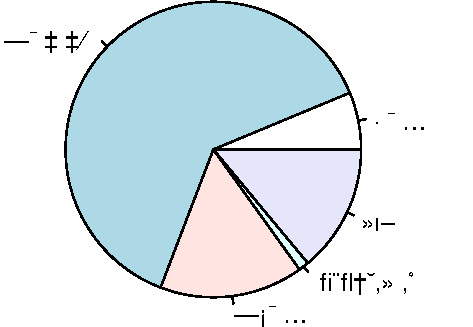
\includegraphics{linear_regression_files/figure-latex/unnamed-chunk-9-1.pdf}

\begin{Shaded}
\begin{Highlighting}[]
\NormalTok{data=}\KeywordTok{data.frame}\NormalTok{(}\DataTypeTok{level=}\NormalTok{bigmu,}\DataTypeTok{data=}\NormalTok{bigy)}
\NormalTok{data$date=}\KeywordTok{seq}\NormalTok{(}\KeywordTok{as.Date}\NormalTok{(}\StringTok{'2010-01-01'}\NormalTok{),}\DataTypeTok{by=}\StringTok{'day'}\NormalTok{,}\DataTypeTok{length.out=}\DecValTok{100}\NormalTok{)}
\NormalTok{d=}\KeywordTok{melt}\NormalTok{(data,}\DataTypeTok{id.vars=}\StringTok{'date'}\NormalTok{)}
\KeywordTok{ggplot}\NormalTok{(d,}\KeywordTok{aes}\NormalTok{(}\DataTypeTok{x=}\NormalTok{date,}\DataTypeTok{y=}\NormalTok{value,}\DataTypeTok{colour=}\NormalTok{variable,}\DataTypeTok{group=}\NormalTok{variable))+}\KeywordTok{geom_line}\NormalTok{()+}\KeywordTok{ggtitle}\NormalTok{(}\StringTok{'Simulated GLM with W/V=0.5'}\NormalTok{)}
\end{Highlighting}
\end{Shaded}

\begin{verbatim}
## Warning in grid.Call(C_textBounds, as.graphicsAnnot(x$label), x$x, x$y, :
## conversion failure on '1月' in 'mbcsToSbcs': dot substituted for <e6>
\end{verbatim}

\begin{verbatim}
## Warning in grid.Call(C_textBounds, as.graphicsAnnot(x$label), x$x, x$y, :
## conversion failure on '1月' in 'mbcsToSbcs': dot substituted for <9c>
\end{verbatim}

\begin{verbatim}
## Warning in grid.Call(C_textBounds, as.graphicsAnnot(x$label), x$x, x$y, :
## conversion failure on '1月' in 'mbcsToSbcs': dot substituted for <88>
\end{verbatim}

\begin{verbatim}
## Warning in grid.Call(C_textBounds, as.graphicsAnnot(x$label), x$x, x$y, :
## conversion failure on '2月' in 'mbcsToSbcs': dot substituted for <e6>
\end{verbatim}

\begin{verbatim}
## Warning in grid.Call(C_textBounds, as.graphicsAnnot(x$label), x$x, x$y, :
## conversion failure on '2月' in 'mbcsToSbcs': dot substituted for <9c>
\end{verbatim}

\begin{verbatim}
## Warning in grid.Call(C_textBounds, as.graphicsAnnot(x$label), x$x, x$y, :
## conversion failure on '2月' in 'mbcsToSbcs': dot substituted for <88>
\end{verbatim}

\begin{verbatim}
## Warning in grid.Call(C_textBounds, as.graphicsAnnot(x$label), x$x, x$y, :
## conversion failure on '3月' in 'mbcsToSbcs': dot substituted for <e6>
\end{verbatim}

\begin{verbatim}
## Warning in grid.Call(C_textBounds, as.graphicsAnnot(x$label), x$x, x$y, :
## conversion failure on '3月' in 'mbcsToSbcs': dot substituted for <9c>
\end{verbatim}

\begin{verbatim}
## Warning in grid.Call(C_textBounds, as.graphicsAnnot(x$label), x$x, x$y, :
## conversion failure on '3月' in 'mbcsToSbcs': dot substituted for <88>
\end{verbatim}

\begin{verbatim}
## Warning in grid.Call(C_textBounds, as.graphicsAnnot(x$label), x$x, x$y, :
## conversion failure on '4月' in 'mbcsToSbcs': dot substituted for <e6>
\end{verbatim}

\begin{verbatim}
## Warning in grid.Call(C_textBounds, as.graphicsAnnot(x$label), x$x, x$y, :
## conversion failure on '4月' in 'mbcsToSbcs': dot substituted for <9c>
\end{verbatim}

\begin{verbatim}
## Warning in grid.Call(C_textBounds, as.graphicsAnnot(x$label), x$x, x$y, :
## conversion failure on '4月' in 'mbcsToSbcs': dot substituted for <88>
\end{verbatim}

\begin{verbatim}
## Warning in grid.Call(C_textBounds, as.graphicsAnnot(x$label), x$x, x$y, :
## conversion failure on '1月' in 'mbcsToSbcs': dot substituted for <e6>
\end{verbatim}

\begin{verbatim}
## Warning in grid.Call(C_textBounds, as.graphicsAnnot(x$label), x$x, x$y, :
## conversion failure on '1月' in 'mbcsToSbcs': dot substituted for <9c>
\end{verbatim}

\begin{verbatim}
## Warning in grid.Call(C_textBounds, as.graphicsAnnot(x$label), x$x, x$y, :
## conversion failure on '1月' in 'mbcsToSbcs': dot substituted for <88>
\end{verbatim}

\begin{verbatim}
## Warning in grid.Call(C_textBounds, as.graphicsAnnot(x$label), x$x, x$y, :
## conversion failure on '2月' in 'mbcsToSbcs': dot substituted for <e6>
\end{verbatim}

\begin{verbatim}
## Warning in grid.Call(C_textBounds, as.graphicsAnnot(x$label), x$x, x$y, :
## conversion failure on '2月' in 'mbcsToSbcs': dot substituted for <9c>
\end{verbatim}

\begin{verbatim}
## Warning in grid.Call(C_textBounds, as.graphicsAnnot(x$label), x$x, x$y, :
## conversion failure on '2月' in 'mbcsToSbcs': dot substituted for <88>
\end{verbatim}

\begin{verbatim}
## Warning in grid.Call(C_textBounds, as.graphicsAnnot(x$label), x$x, x$y, :
## conversion failure on '3月' in 'mbcsToSbcs': dot substituted for <e6>
\end{verbatim}

\begin{verbatim}
## Warning in grid.Call(C_textBounds, as.graphicsAnnot(x$label), x$x, x$y, :
## conversion failure on '3月' in 'mbcsToSbcs': dot substituted for <9c>
\end{verbatim}

\begin{verbatim}
## Warning in grid.Call(C_textBounds, as.graphicsAnnot(x$label), x$x, x$y, :
## conversion failure on '3月' in 'mbcsToSbcs': dot substituted for <88>
\end{verbatim}

\begin{verbatim}
## Warning in grid.Call(C_textBounds, as.graphicsAnnot(x$label), x$x, x$y, :
## conversion failure on '4月' in 'mbcsToSbcs': dot substituted for <e6>
\end{verbatim}

\begin{verbatim}
## Warning in grid.Call(C_textBounds, as.graphicsAnnot(x$label), x$x, x$y, :
## conversion failure on '4月' in 'mbcsToSbcs': dot substituted for <9c>
\end{verbatim}

\begin{verbatim}
## Warning in grid.Call(C_textBounds, as.graphicsAnnot(x$label), x$x, x$y, :
## conversion failure on '4月' in 'mbcsToSbcs': dot substituted for <88>
\end{verbatim}

\begin{verbatim}
## Warning in grid.Call(C_textBounds, as.graphicsAnnot(x$label), x$x, x$y, :
## conversion failure on '1月' in 'mbcsToSbcs': dot substituted for <e6>
\end{verbatim}

\begin{verbatim}
## Warning in grid.Call(C_textBounds, as.graphicsAnnot(x$label), x$x, x$y, :
## conversion failure on '1月' in 'mbcsToSbcs': dot substituted for <9c>
\end{verbatim}

\begin{verbatim}
## Warning in grid.Call(C_textBounds, as.graphicsAnnot(x$label), x$x, x$y, :
## conversion failure on '1月' in 'mbcsToSbcs': dot substituted for <88>
\end{verbatim}

\begin{verbatim}
## Warning in grid.Call(C_textBounds, as.graphicsAnnot(x$label), x$x, x$y, :
## conversion failure on '2月' in 'mbcsToSbcs': dot substituted for <e6>
\end{verbatim}

\begin{verbatim}
## Warning in grid.Call(C_textBounds, as.graphicsAnnot(x$label), x$x, x$y, :
## conversion failure on '2月' in 'mbcsToSbcs': dot substituted for <9c>
\end{verbatim}

\begin{verbatim}
## Warning in grid.Call(C_textBounds, as.graphicsAnnot(x$label), x$x, x$y, :
## conversion failure on '2月' in 'mbcsToSbcs': dot substituted for <88>
\end{verbatim}

\begin{verbatim}
## Warning in grid.Call(C_textBounds, as.graphicsAnnot(x$label), x$x, x$y, :
## conversion failure on '3月' in 'mbcsToSbcs': dot substituted for <e6>
\end{verbatim}

\begin{verbatim}
## Warning in grid.Call(C_textBounds, as.graphicsAnnot(x$label), x$x, x$y, :
## conversion failure on '3月' in 'mbcsToSbcs': dot substituted for <9c>
\end{verbatim}

\begin{verbatim}
## Warning in grid.Call(C_textBounds, as.graphicsAnnot(x$label), x$x, x$y, :
## conversion failure on '3月' in 'mbcsToSbcs': dot substituted for <88>
\end{verbatim}

\begin{verbatim}
## Warning in grid.Call(C_textBounds, as.graphicsAnnot(x$label), x$x, x$y, :
## conversion failure on '4月' in 'mbcsToSbcs': dot substituted for <e6>
\end{verbatim}

\begin{verbatim}
## Warning in grid.Call(C_textBounds, as.graphicsAnnot(x$label), x$x, x$y, :
## conversion failure on '4月' in 'mbcsToSbcs': dot substituted for <9c>
\end{verbatim}

\begin{verbatim}
## Warning in grid.Call(C_textBounds, as.graphicsAnnot(x$label), x$x, x$y, :
## conversion failure on '4月' in 'mbcsToSbcs': dot substituted for <88>
\end{verbatim}

\begin{verbatim}
## Warning in grid.Call(C_textBounds, as.graphicsAnnot(x$label), x$x, x$y, :
## conversion failure on '1月' in 'mbcsToSbcs': dot substituted for <e6>
\end{verbatim}

\begin{verbatim}
## Warning in grid.Call(C_textBounds, as.graphicsAnnot(x$label), x$x, x$y, :
## conversion failure on '1月' in 'mbcsToSbcs': dot substituted for <9c>
\end{verbatim}

\begin{verbatim}
## Warning in grid.Call(C_textBounds, as.graphicsAnnot(x$label), x$x, x$y, :
## conversion failure on '1月' in 'mbcsToSbcs': dot substituted for <88>
\end{verbatim}

\begin{verbatim}
## Warning in grid.Call(C_textBounds, as.graphicsAnnot(x$label), x$x, x$y, :
## conversion failure on '2月' in 'mbcsToSbcs': dot substituted for <e6>
\end{verbatim}

\begin{verbatim}
## Warning in grid.Call(C_textBounds, as.graphicsAnnot(x$label), x$x, x$y, :
## conversion failure on '2月' in 'mbcsToSbcs': dot substituted for <9c>
\end{verbatim}

\begin{verbatim}
## Warning in grid.Call(C_textBounds, as.graphicsAnnot(x$label), x$x, x$y, :
## conversion failure on '2月' in 'mbcsToSbcs': dot substituted for <88>
\end{verbatim}

\begin{verbatim}
## Warning in grid.Call(C_textBounds, as.graphicsAnnot(x$label), x$x, x$y, :
## conversion failure on '3月' in 'mbcsToSbcs': dot substituted for <e6>
\end{verbatim}

\begin{verbatim}
## Warning in grid.Call(C_textBounds, as.graphicsAnnot(x$label), x$x, x$y, :
## conversion failure on '3月' in 'mbcsToSbcs': dot substituted for <9c>
\end{verbatim}

\begin{verbatim}
## Warning in grid.Call(C_textBounds, as.graphicsAnnot(x$label), x$x, x$y, :
## conversion failure on '3月' in 'mbcsToSbcs': dot substituted for <88>
\end{verbatim}

\begin{verbatim}
## Warning in grid.Call(C_textBounds, as.graphicsAnnot(x$label), x$x, x$y, :
## conversion failure on '4月' in 'mbcsToSbcs': dot substituted for <e6>
\end{verbatim}

\begin{verbatim}
## Warning in grid.Call(C_textBounds, as.graphicsAnnot(x$label), x$x, x$y, :
## conversion failure on '4月' in 'mbcsToSbcs': dot substituted for <9c>
\end{verbatim}

\begin{verbatim}
## Warning in grid.Call(C_textBounds, as.graphicsAnnot(x$label), x$x, x$y, :
## conversion failure on '4月' in 'mbcsToSbcs': dot substituted for <88>
\end{verbatim}

\begin{verbatim}
## Warning in grid.Call(C_textBounds, as.graphicsAnnot(x$label), x$x, x$y, :
## conversion failure on '1月' in 'mbcsToSbcs': dot substituted for <e6>
\end{verbatim}

\begin{verbatim}
## Warning in grid.Call(C_textBounds, as.graphicsAnnot(x$label), x$x, x$y, :
## conversion failure on '1月' in 'mbcsToSbcs': dot substituted for <9c>
\end{verbatim}

\begin{verbatim}
## Warning in grid.Call(C_textBounds, as.graphicsAnnot(x$label), x$x, x$y, :
## conversion failure on '1月' in 'mbcsToSbcs': dot substituted for <88>
\end{verbatim}

\begin{verbatim}
## Warning in grid.Call(C_textBounds, as.graphicsAnnot(x$label), x$x, x$y, :
## conversion failure on '2月' in 'mbcsToSbcs': dot substituted for <e6>
\end{verbatim}

\begin{verbatim}
## Warning in grid.Call(C_textBounds, as.graphicsAnnot(x$label), x$x, x$y, :
## conversion failure on '2月' in 'mbcsToSbcs': dot substituted for <9c>
\end{verbatim}

\begin{verbatim}
## Warning in grid.Call(C_textBounds, as.graphicsAnnot(x$label), x$x, x$y, :
## conversion failure on '2月' in 'mbcsToSbcs': dot substituted for <88>
\end{verbatim}

\begin{verbatim}
## Warning in grid.Call(C_textBounds, as.graphicsAnnot(x$label), x$x, x$y, :
## conversion failure on '3月' in 'mbcsToSbcs': dot substituted for <e6>
\end{verbatim}

\begin{verbatim}
## Warning in grid.Call(C_textBounds, as.graphicsAnnot(x$label), x$x, x$y, :
## conversion failure on '3月' in 'mbcsToSbcs': dot substituted for <9c>
\end{verbatim}

\begin{verbatim}
## Warning in grid.Call(C_textBounds, as.graphicsAnnot(x$label), x$x, x$y, :
## conversion failure on '3月' in 'mbcsToSbcs': dot substituted for <88>
\end{verbatim}

\begin{verbatim}
## Warning in grid.Call(C_textBounds, as.graphicsAnnot(x$label), x$x, x$y, :
## conversion failure on '4月' in 'mbcsToSbcs': dot substituted for <e6>
\end{verbatim}

\begin{verbatim}
## Warning in grid.Call(C_textBounds, as.graphicsAnnot(x$label), x$x, x$y, :
## conversion failure on '4月' in 'mbcsToSbcs': dot substituted for <9c>
\end{verbatim}

\begin{verbatim}
## Warning in grid.Call(C_textBounds, as.graphicsAnnot(x$label), x$x, x$y, :
## conversion failure on '4月' in 'mbcsToSbcs': dot substituted for <88>
\end{verbatim}

\begin{verbatim}
## Warning in grid.Call(C_textBounds, as.graphicsAnnot(x$label), x$x, x$y, :
## conversion failure on '1月' in 'mbcsToSbcs': dot substituted for <e6>
\end{verbatim}

\begin{verbatim}
## Warning in grid.Call(C_textBounds, as.graphicsAnnot(x$label), x$x, x$y, :
## conversion failure on '1月' in 'mbcsToSbcs': dot substituted for <9c>
\end{verbatim}

\begin{verbatim}
## Warning in grid.Call(C_textBounds, as.graphicsAnnot(x$label), x$x, x$y, :
## conversion failure on '1月' in 'mbcsToSbcs': dot substituted for <88>
\end{verbatim}

\begin{verbatim}
## Warning in grid.Call(C_textBounds, as.graphicsAnnot(x$label), x$x, x$y, :
## conversion failure on '2月' in 'mbcsToSbcs': dot substituted for <e6>
\end{verbatim}

\begin{verbatim}
## Warning in grid.Call(C_textBounds, as.graphicsAnnot(x$label), x$x, x$y, :
## conversion failure on '2月' in 'mbcsToSbcs': dot substituted for <9c>
\end{verbatim}

\begin{verbatim}
## Warning in grid.Call(C_textBounds, as.graphicsAnnot(x$label), x$x, x$y, :
## conversion failure on '2月' in 'mbcsToSbcs': dot substituted for <88>
\end{verbatim}

\begin{verbatim}
## Warning in grid.Call(C_textBounds, as.graphicsAnnot(x$label), x$x, x$y, :
## conversion failure on '3月' in 'mbcsToSbcs': dot substituted for <e6>
\end{verbatim}

\begin{verbatim}
## Warning in grid.Call(C_textBounds, as.graphicsAnnot(x$label), x$x, x$y, :
## conversion failure on '3月' in 'mbcsToSbcs': dot substituted for <9c>
\end{verbatim}

\begin{verbatim}
## Warning in grid.Call(C_textBounds, as.graphicsAnnot(x$label), x$x, x$y, :
## conversion failure on '3月' in 'mbcsToSbcs': dot substituted for <88>
\end{verbatim}

\begin{verbatim}
## Warning in grid.Call(C_textBounds, as.graphicsAnnot(x$label), x$x, x$y, :
## conversion failure on '4月' in 'mbcsToSbcs': dot substituted for <e6>
\end{verbatim}

\begin{verbatim}
## Warning in grid.Call(C_textBounds, as.graphicsAnnot(x$label), x$x, x$y, :
## conversion failure on '4月' in 'mbcsToSbcs': dot substituted for <9c>
\end{verbatim}

\begin{verbatim}
## Warning in grid.Call(C_textBounds, as.graphicsAnnot(x$label), x$x, x$y, :
## conversion failure on '4月' in 'mbcsToSbcs': dot substituted for <88>
\end{verbatim}

\begin{verbatim}
## Warning in grid.Call(C_textBounds, as.graphicsAnnot(x$label), x$x, x$y, :
## conversion failure on '1月' in 'mbcsToSbcs': dot substituted for <e6>
\end{verbatim}

\begin{verbatim}
## Warning in grid.Call(C_textBounds, as.graphicsAnnot(x$label), x$x, x$y, :
## conversion failure on '1月' in 'mbcsToSbcs': dot substituted for <9c>
\end{verbatim}

\begin{verbatim}
## Warning in grid.Call(C_textBounds, as.graphicsAnnot(x$label), x$x, x$y, :
## conversion failure on '1月' in 'mbcsToSbcs': dot substituted for <88>
\end{verbatim}

\begin{verbatim}
## Warning in grid.Call(C_textBounds, as.graphicsAnnot(x$label), x$x, x$y, :
## conversion failure on '2月' in 'mbcsToSbcs': dot substituted for <e6>
\end{verbatim}

\begin{verbatim}
## Warning in grid.Call(C_textBounds, as.graphicsAnnot(x$label), x$x, x$y, :
## conversion failure on '2月' in 'mbcsToSbcs': dot substituted for <9c>
\end{verbatim}

\begin{verbatim}
## Warning in grid.Call(C_textBounds, as.graphicsAnnot(x$label), x$x, x$y, :
## conversion failure on '2月' in 'mbcsToSbcs': dot substituted for <88>
\end{verbatim}

\begin{verbatim}
## Warning in grid.Call(C_textBounds, as.graphicsAnnot(x$label), x$x, x$y, :
## conversion failure on '3月' in 'mbcsToSbcs': dot substituted for <e6>
\end{verbatim}

\begin{verbatim}
## Warning in grid.Call(C_textBounds, as.graphicsAnnot(x$label), x$x, x$y, :
## conversion failure on '3月' in 'mbcsToSbcs': dot substituted for <9c>
\end{verbatim}

\begin{verbatim}
## Warning in grid.Call(C_textBounds, as.graphicsAnnot(x$label), x$x, x$y, :
## conversion failure on '3月' in 'mbcsToSbcs': dot substituted for <88>
\end{verbatim}

\begin{verbatim}
## Warning in grid.Call(C_textBounds, as.graphicsAnnot(x$label), x$x, x$y, :
## conversion failure on '4月' in 'mbcsToSbcs': dot substituted for <e6>
\end{verbatim}

\begin{verbatim}
## Warning in grid.Call(C_textBounds, as.graphicsAnnot(x$label), x$x, x$y, :
## conversion failure on '4月' in 'mbcsToSbcs': dot substituted for <9c>
\end{verbatim}

\begin{verbatim}
## Warning in grid.Call(C_textBounds, as.graphicsAnnot(x$label), x$x, x$y, :
## conversion failure on '4月' in 'mbcsToSbcs': dot substituted for <88>
\end{verbatim}

\begin{verbatim}
## Warning in grid.Call(C_textBounds, as.graphicsAnnot(x$label), x$x, x$y, :
## conversion failure on '1月' in 'mbcsToSbcs': dot substituted for <e6>
\end{verbatim}

\begin{verbatim}
## Warning in grid.Call(C_textBounds, as.graphicsAnnot(x$label), x$x, x$y, :
## conversion failure on '1月' in 'mbcsToSbcs': dot substituted for <9c>
\end{verbatim}

\begin{verbatim}
## Warning in grid.Call(C_textBounds, as.graphicsAnnot(x$label), x$x, x$y, :
## conversion failure on '1月' in 'mbcsToSbcs': dot substituted for <88>
\end{verbatim}

\begin{verbatim}
## Warning in grid.Call(C_textBounds, as.graphicsAnnot(x$label), x$x, x$y, :
## conversion failure on '2月' in 'mbcsToSbcs': dot substituted for <e6>
\end{verbatim}

\begin{verbatim}
## Warning in grid.Call(C_textBounds, as.graphicsAnnot(x$label), x$x, x$y, :
## conversion failure on '2月' in 'mbcsToSbcs': dot substituted for <9c>
\end{verbatim}

\begin{verbatim}
## Warning in grid.Call(C_textBounds, as.graphicsAnnot(x$label), x$x, x$y, :
## conversion failure on '2月' in 'mbcsToSbcs': dot substituted for <88>
\end{verbatim}

\begin{verbatim}
## Warning in grid.Call(C_textBounds, as.graphicsAnnot(x$label), x$x, x$y, :
## conversion failure on '3月' in 'mbcsToSbcs': dot substituted for <e6>
\end{verbatim}

\begin{verbatim}
## Warning in grid.Call(C_textBounds, as.graphicsAnnot(x$label), x$x, x$y, :
## conversion failure on '3月' in 'mbcsToSbcs': dot substituted for <9c>
\end{verbatim}

\begin{verbatim}
## Warning in grid.Call(C_textBounds, as.graphicsAnnot(x$label), x$x, x$y, :
## conversion failure on '3月' in 'mbcsToSbcs': dot substituted for <88>
\end{verbatim}

\begin{verbatim}
## Warning in grid.Call(C_textBounds, as.graphicsAnnot(x$label), x$x, x$y, :
## conversion failure on '4月' in 'mbcsToSbcs': dot substituted for <e6>
\end{verbatim}

\begin{verbatim}
## Warning in grid.Call(C_textBounds, as.graphicsAnnot(x$label), x$x, x$y, :
## conversion failure on '4月' in 'mbcsToSbcs': dot substituted for <9c>
\end{verbatim}

\begin{verbatim}
## Warning in grid.Call(C_textBounds, as.graphicsAnnot(x$label), x$x, x$y, :
## conversion failure on '4月' in 'mbcsToSbcs': dot substituted for <88>
\end{verbatim}

\begin{verbatim}
## Warning in grid.Call(C_textBounds, as.graphicsAnnot(x$label), x$x, x$y, :
## conversion failure on '1月' in 'mbcsToSbcs': dot substituted for <e6>
\end{verbatim}

\begin{verbatim}
## Warning in grid.Call(C_textBounds, as.graphicsAnnot(x$label), x$x, x$y, :
## conversion failure on '1月' in 'mbcsToSbcs': dot substituted for <9c>
\end{verbatim}

\begin{verbatim}
## Warning in grid.Call(C_textBounds, as.graphicsAnnot(x$label), x$x, x$y, :
## conversion failure on '1月' in 'mbcsToSbcs': dot substituted for <88>
\end{verbatim}

\begin{verbatim}
## Warning in grid.Call(C_textBounds, as.graphicsAnnot(x$label), x$x, x$y, :
## conversion failure on '2月' in 'mbcsToSbcs': dot substituted for <e6>
\end{verbatim}

\begin{verbatim}
## Warning in grid.Call(C_textBounds, as.graphicsAnnot(x$label), x$x, x$y, :
## conversion failure on '2月' in 'mbcsToSbcs': dot substituted for <9c>
\end{verbatim}

\begin{verbatim}
## Warning in grid.Call(C_textBounds, as.graphicsAnnot(x$label), x$x, x$y, :
## conversion failure on '2月' in 'mbcsToSbcs': dot substituted for <88>
\end{verbatim}

\begin{verbatim}
## Warning in grid.Call(C_textBounds, as.graphicsAnnot(x$label), x$x, x$y, :
## conversion failure on '3月' in 'mbcsToSbcs': dot substituted for <e6>
\end{verbatim}

\begin{verbatim}
## Warning in grid.Call(C_textBounds, as.graphicsAnnot(x$label), x$x, x$y, :
## conversion failure on '3月' in 'mbcsToSbcs': dot substituted for <9c>
\end{verbatim}

\begin{verbatim}
## Warning in grid.Call(C_textBounds, as.graphicsAnnot(x$label), x$x, x$y, :
## conversion failure on '3月' in 'mbcsToSbcs': dot substituted for <88>
\end{verbatim}

\begin{verbatim}
## Warning in grid.Call(C_textBounds, as.graphicsAnnot(x$label), x$x, x$y, :
## conversion failure on '4月' in 'mbcsToSbcs': dot substituted for <e6>
\end{verbatim}

\begin{verbatim}
## Warning in grid.Call(C_textBounds, as.graphicsAnnot(x$label), x$x, x$y, :
## conversion failure on '4月' in 'mbcsToSbcs': dot substituted for <9c>
\end{verbatim}

\begin{verbatim}
## Warning in grid.Call(C_textBounds, as.graphicsAnnot(x$label), x$x, x$y, :
## conversion failure on '4月' in 'mbcsToSbcs': dot substituted for <88>
\end{verbatim}

\begin{verbatim}
## Warning in grid.Call(C_textBounds, as.graphicsAnnot(x$label), x$x, x$y, :
## conversion failure on '1月' in 'mbcsToSbcs': dot substituted for <e6>
\end{verbatim}

\begin{verbatim}
## Warning in grid.Call(C_textBounds, as.graphicsAnnot(x$label), x$x, x$y, :
## conversion failure on '1月' in 'mbcsToSbcs': dot substituted for <9c>
\end{verbatim}

\begin{verbatim}
## Warning in grid.Call(C_textBounds, as.graphicsAnnot(x$label), x$x, x$y, :
## conversion failure on '1月' in 'mbcsToSbcs': dot substituted for <88>
\end{verbatim}

\begin{verbatim}
## Warning in grid.Call(C_textBounds, as.graphicsAnnot(x$label), x$x, x$y, :
## conversion failure on '2月' in 'mbcsToSbcs': dot substituted for <e6>
\end{verbatim}

\begin{verbatim}
## Warning in grid.Call(C_textBounds, as.graphicsAnnot(x$label), x$x, x$y, :
## conversion failure on '2月' in 'mbcsToSbcs': dot substituted for <9c>
\end{verbatim}

\begin{verbatim}
## Warning in grid.Call(C_textBounds, as.graphicsAnnot(x$label), x$x, x$y, :
## conversion failure on '2月' in 'mbcsToSbcs': dot substituted for <88>
\end{verbatim}

\begin{verbatim}
## Warning in grid.Call(C_textBounds, as.graphicsAnnot(x$label), x$x, x$y, :
## conversion failure on '3月' in 'mbcsToSbcs': dot substituted for <e6>
\end{verbatim}

\begin{verbatim}
## Warning in grid.Call(C_textBounds, as.graphicsAnnot(x$label), x$x, x$y, :
## conversion failure on '3月' in 'mbcsToSbcs': dot substituted for <9c>
\end{verbatim}

\begin{verbatim}
## Warning in grid.Call(C_textBounds, as.graphicsAnnot(x$label), x$x, x$y, :
## conversion failure on '3月' in 'mbcsToSbcs': dot substituted for <88>
\end{verbatim}

\begin{verbatim}
## Warning in grid.Call(C_textBounds, as.graphicsAnnot(x$label), x$x, x$y, :
## conversion failure on '4月' in 'mbcsToSbcs': dot substituted for <e6>
\end{verbatim}

\begin{verbatim}
## Warning in grid.Call(C_textBounds, as.graphicsAnnot(x$label), x$x, x$y, :
## conversion failure on '4月' in 'mbcsToSbcs': dot substituted for <9c>
\end{verbatim}

\begin{verbatim}
## Warning in grid.Call(C_textBounds, as.graphicsAnnot(x$label), x$x, x$y, :
## conversion failure on '4月' in 'mbcsToSbcs': dot substituted for <88>
\end{verbatim}

\begin{verbatim}
## Warning in grid.Call(C_textBounds, as.graphicsAnnot(x$label), x$x, x$y, :
## conversion failure on '1月' in 'mbcsToSbcs': dot substituted for <e6>
\end{verbatim}

\begin{verbatim}
## Warning in grid.Call(C_textBounds, as.graphicsAnnot(x$label), x$x, x$y, :
## conversion failure on '1月' in 'mbcsToSbcs': dot substituted for <9c>
\end{verbatim}

\begin{verbatim}
## Warning in grid.Call(C_textBounds, as.graphicsAnnot(x$label), x$x, x$y, :
## conversion failure on '1月' in 'mbcsToSbcs': dot substituted for <88>
\end{verbatim}

\begin{verbatim}
## Warning in grid.Call(C_textBounds, as.graphicsAnnot(x$label), x$x, x$y, :
## conversion failure on '2月' in 'mbcsToSbcs': dot substituted for <e6>
\end{verbatim}

\begin{verbatim}
## Warning in grid.Call(C_textBounds, as.graphicsAnnot(x$label), x$x, x$y, :
## conversion failure on '2月' in 'mbcsToSbcs': dot substituted for <9c>
\end{verbatim}

\begin{verbatim}
## Warning in grid.Call(C_textBounds, as.graphicsAnnot(x$label), x$x, x$y, :
## conversion failure on '2月' in 'mbcsToSbcs': dot substituted for <88>
\end{verbatim}

\begin{verbatim}
## Warning in grid.Call(C_textBounds, as.graphicsAnnot(x$label), x$x, x$y, :
## conversion failure on '3月' in 'mbcsToSbcs': dot substituted for <e6>
\end{verbatim}

\begin{verbatim}
## Warning in grid.Call(C_textBounds, as.graphicsAnnot(x$label), x$x, x$y, :
## conversion failure on '3月' in 'mbcsToSbcs': dot substituted for <9c>
\end{verbatim}

\begin{verbatim}
## Warning in grid.Call(C_textBounds, as.graphicsAnnot(x$label), x$x, x$y, :
## conversion failure on '3月' in 'mbcsToSbcs': dot substituted for <88>
\end{verbatim}

\begin{verbatim}
## Warning in grid.Call(C_textBounds, as.graphicsAnnot(x$label), x$x, x$y, :
## conversion failure on '4月' in 'mbcsToSbcs': dot substituted for <e6>
\end{verbatim}

\begin{verbatim}
## Warning in grid.Call(C_textBounds, as.graphicsAnnot(x$label), x$x, x$y, :
## conversion failure on '4月' in 'mbcsToSbcs': dot substituted for <9c>
\end{verbatim}

\begin{verbatim}
## Warning in grid.Call(C_textBounds, as.graphicsAnnot(x$label), x$x, x$y, :
## conversion failure on '4月' in 'mbcsToSbcs': dot substituted for <88>
\end{verbatim}

\begin{verbatim}
## Warning in grid.Call(C_textBounds, as.graphicsAnnot(x$label), x$x, x$y, :
## conversion failure on '1月' in 'mbcsToSbcs': dot substituted for <e6>
\end{verbatim}

\begin{verbatim}
## Warning in grid.Call(C_textBounds, as.graphicsAnnot(x$label), x$x, x$y, :
## conversion failure on '1月' in 'mbcsToSbcs': dot substituted for <9c>
\end{verbatim}

\begin{verbatim}
## Warning in grid.Call(C_textBounds, as.graphicsAnnot(x$label), x$x, x$y, :
## conversion failure on '1月' in 'mbcsToSbcs': dot substituted for <88>
\end{verbatim}

\begin{verbatim}
## Warning in grid.Call(C_textBounds, as.graphicsAnnot(x$label), x$x, x$y, :
## conversion failure on '2月' in 'mbcsToSbcs': dot substituted for <e6>
\end{verbatim}

\begin{verbatim}
## Warning in grid.Call(C_textBounds, as.graphicsAnnot(x$label), x$x, x$y, :
## conversion failure on '2月' in 'mbcsToSbcs': dot substituted for <9c>
\end{verbatim}

\begin{verbatim}
## Warning in grid.Call(C_textBounds, as.graphicsAnnot(x$label), x$x, x$y, :
## conversion failure on '2月' in 'mbcsToSbcs': dot substituted for <88>
\end{verbatim}

\begin{verbatim}
## Warning in grid.Call(C_textBounds, as.graphicsAnnot(x$label), x$x, x$y, :
## conversion failure on '3月' in 'mbcsToSbcs': dot substituted for <e6>
\end{verbatim}

\begin{verbatim}
## Warning in grid.Call(C_textBounds, as.graphicsAnnot(x$label), x$x, x$y, :
## conversion failure on '3月' in 'mbcsToSbcs': dot substituted for <9c>
\end{verbatim}

\begin{verbatim}
## Warning in grid.Call(C_textBounds, as.graphicsAnnot(x$label), x$x, x$y, :
## conversion failure on '3月' in 'mbcsToSbcs': dot substituted for <88>
\end{verbatim}

\begin{verbatim}
## Warning in grid.Call(C_textBounds, as.graphicsAnnot(x$label), x$x, x$y, :
## conversion failure on '4月' in 'mbcsToSbcs': dot substituted for <e6>
\end{verbatim}

\begin{verbatim}
## Warning in grid.Call(C_textBounds, as.graphicsAnnot(x$label), x$x, x$y, :
## conversion failure on '4月' in 'mbcsToSbcs': dot substituted for <9c>
\end{verbatim}

\begin{verbatim}
## Warning in grid.Call(C_textBounds, as.graphicsAnnot(x$label), x$x, x$y, :
## conversion failure on '4月' in 'mbcsToSbcs': dot substituted for <88>
\end{verbatim}

\begin{verbatim}
## Warning in grid.Call(C_textBounds, as.graphicsAnnot(x$label), x$x, x$y, :
## conversion failure on '1月' in 'mbcsToSbcs': dot substituted for <e6>
\end{verbatim}

\begin{verbatim}
## Warning in grid.Call(C_textBounds, as.graphicsAnnot(x$label), x$x, x$y, :
## conversion failure on '1月' in 'mbcsToSbcs': dot substituted for <9c>
\end{verbatim}

\begin{verbatim}
## Warning in grid.Call(C_textBounds, as.graphicsAnnot(x$label), x$x, x$y, :
## conversion failure on '1月' in 'mbcsToSbcs': dot substituted for <88>
\end{verbatim}

\begin{verbatim}
## Warning in grid.Call(C_textBounds, as.graphicsAnnot(x$label), x$x, x$y, :
## conversion failure on '2月' in 'mbcsToSbcs': dot substituted for <e6>
\end{verbatim}

\begin{verbatim}
## Warning in grid.Call(C_textBounds, as.graphicsAnnot(x$label), x$x, x$y, :
## conversion failure on '2月' in 'mbcsToSbcs': dot substituted for <9c>
\end{verbatim}

\begin{verbatim}
## Warning in grid.Call(C_textBounds, as.graphicsAnnot(x$label), x$x, x$y, :
## conversion failure on '2月' in 'mbcsToSbcs': dot substituted for <88>
\end{verbatim}

\begin{verbatim}
## Warning in grid.Call(C_textBounds, as.graphicsAnnot(x$label), x$x, x$y, :
## conversion failure on '3月' in 'mbcsToSbcs': dot substituted for <e6>
\end{verbatim}

\begin{verbatim}
## Warning in grid.Call(C_textBounds, as.graphicsAnnot(x$label), x$x, x$y, :
## conversion failure on '3月' in 'mbcsToSbcs': dot substituted for <9c>
\end{verbatim}

\begin{verbatim}
## Warning in grid.Call(C_textBounds, as.graphicsAnnot(x$label), x$x, x$y, :
## conversion failure on '3月' in 'mbcsToSbcs': dot substituted for <88>
\end{verbatim}

\begin{verbatim}
## Warning in grid.Call(C_textBounds, as.graphicsAnnot(x$label), x$x, x$y, :
## conversion failure on '4月' in 'mbcsToSbcs': dot substituted for <e6>
\end{verbatim}

\begin{verbatim}
## Warning in grid.Call(C_textBounds, as.graphicsAnnot(x$label), x$x, x$y, :
## conversion failure on '4月' in 'mbcsToSbcs': dot substituted for <9c>
\end{verbatim}

\begin{verbatim}
## Warning in grid.Call(C_textBounds, as.graphicsAnnot(x$label), x$x, x$y, :
## conversion failure on '4月' in 'mbcsToSbcs': dot substituted for <88>
\end{verbatim}

\begin{verbatim}
## Warning in grid.Call.graphics(C_text, as.graphicsAnnot(x$label), x$x, x
## $y, : conversion failure on '1月' in 'mbcsToSbcs': dot substituted for <e6>
\end{verbatim}

\begin{verbatim}
## Warning in grid.Call.graphics(C_text, as.graphicsAnnot(x$label), x$x, x
## $y, : conversion failure on '1月' in 'mbcsToSbcs': dot substituted for <9c>
\end{verbatim}

\begin{verbatim}
## Warning in grid.Call.graphics(C_text, as.graphicsAnnot(x$label), x$x, x
## $y, : conversion failure on '1月' in 'mbcsToSbcs': dot substituted for <88>
\end{verbatim}

\begin{verbatim}
## Warning in grid.Call.graphics(C_text, as.graphicsAnnot(x$label), x$x, x
## $y, : conversion failure on '2月' in 'mbcsToSbcs': dot substituted for <e6>
\end{verbatim}

\begin{verbatim}
## Warning in grid.Call.graphics(C_text, as.graphicsAnnot(x$label), x$x, x
## $y, : conversion failure on '2月' in 'mbcsToSbcs': dot substituted for <9c>
\end{verbatim}

\begin{verbatim}
## Warning in grid.Call.graphics(C_text, as.graphicsAnnot(x$label), x$x, x
## $y, : conversion failure on '2月' in 'mbcsToSbcs': dot substituted for <88>
\end{verbatim}

\begin{verbatim}
## Warning in grid.Call.graphics(C_text, as.graphicsAnnot(x$label), x$x, x
## $y, : conversion failure on '3月' in 'mbcsToSbcs': dot substituted for <e6>
\end{verbatim}

\begin{verbatim}
## Warning in grid.Call.graphics(C_text, as.graphicsAnnot(x$label), x$x, x
## $y, : conversion failure on '3月' in 'mbcsToSbcs': dot substituted for <9c>
\end{verbatim}

\begin{verbatim}
## Warning in grid.Call.graphics(C_text, as.graphicsAnnot(x$label), x$x, x
## $y, : conversion failure on '3月' in 'mbcsToSbcs': dot substituted for <88>
\end{verbatim}

\begin{verbatim}
## Warning in grid.Call.graphics(C_text, as.graphicsAnnot(x$label), x$x, x
## $y, : conversion failure on '4月' in 'mbcsToSbcs': dot substituted for <e6>
\end{verbatim}

\begin{verbatim}
## Warning in grid.Call.graphics(C_text, as.graphicsAnnot(x$label), x$x, x
## $y, : conversion failure on '4月' in 'mbcsToSbcs': dot substituted for <9c>
\end{verbatim}

\begin{verbatim}
## Warning in grid.Call.graphics(C_text, as.graphicsAnnot(x$label), x$x, x
## $y, : conversion failure on '4月' in 'mbcsToSbcs': dot substituted for <88>
\end{verbatim}

\includegraphics{linear_regression_files/figure-latex/unnamed-chunk-9-2.pdf}

显然当\(\frac{W}{V}=0.5\),图形显示,我们建模的假设------局部稳定------并不满足了。此时使用这个模型进行预测不会有什么稳妥的结果。

关于以上的动态线性模型,有着如下的结论:

\begin{enumerate}
\def\labelenumi{\arabic{enumi}.}
\tightlist
\item
  系统状态\(\theta_{t-1}\)的后验概率:
  \((\theta_{t-1}|D_{t-1})\sim N(m_{t-1},C_{t-1})\)
\item
  系统状态\(\theta_{t}\)的先验概率:
  \((\theta_t|D_{t-1})\sim N(m_{t-1},R_t)\),其中\(R_t = C_{t-1}+W_t\)
\item
  1步预测:
  \((Y_t|D_{t-1})\sim N(f_t,Q_t)\),其中\(f_t = m_{t-1}\),\(Q_t=R_t + V_t\)
\item
  系统状态\(\theta_t\)的后验概率:
  \((\theta_t|D_t)\sim N(m_t,C_t)\),其中\(m_t = m_{t-1} + A_t e_t\),\(C_t = A_tV_t\),\(A_t = R_t/Q_t\)以及\(e_t=Y_t-f_t\)
\end{enumerate}

前三条性质都属于平常的贝叶斯概率的东西,第四条性质跟前三条形成了递归的关系。
\[
(Y_t|\theta_t,D_{t-1})\sim N(\theta_t,V_t) \\
(\theta_t|D_{t-1})\sim N(m_{t-1},R_t)
\] 并且,\(D_t = \{ Y_t,D_{t-1}\}\),所以 \[
p(y_t|\theta_t,D_{t-1})=\frac{p(y_t,\theta_t,D_{t-1})}{p(\theta_t,D_{t-1})}=\frac{p(\theta_t,D_{t})}{p(D_{t-1})p(\theta_t|D_{t-1})}=\frac{p(\theta_t|D_t)p(D_t)}{p(D_{t-1})p(\theta_t|D_{t-1})}
\] 可得 \[
p(\theta_t|D_t)=\frac{p(\theta_t|D_{t-1})p(y_t|\theta_t,D_{t-1})}{p(D_t)/p(D_{t-1})}=\frac{p(\theta_t|D_{t-1})p(y_t|\theta_t,D_{t-1})}{p(y_t|D_{t-1})}
\] 只关注跟\(\theta_t\)相关的项目,因此 \[
p(\theta_t|D_t)\propto p(\theta_t|D_{t-1})p(y_t|\theta_t,D_{t-1})\propto \exp[-(\theta_t-m_{t-1})^2/(2R_t) - (y_t-\theta_t)^2/(2V_t)]
\] 进一步,

\begin{eqnarray*}
2\ln(p(\theta_t|D_t))&=&k_1 -(\theta_t - m_{t-1})^2R_t^{-1}-(y_t-\theta_t)^2V_t^{-1} \\
                     &=&k_2 -(R_t^{-1}+V_t^{-1})\theta_t^2+2(R_t^{-1}m_{t-1}+V_t^{-1}y_t)\theta_t
\end{eqnarray*}

那么看看,稍微复杂一点的动态CAPM模型。 \[
  r_{i,t} - r_{f,t} = \alpha_{i,t} + \beta_{i,t} (r_{m,t}-r_{f,t})+\epsilon_{i,t}
\]

\begin{Shaded}
\begin{Highlighting}[]
\KeywordTok{require}\NormalTok{(dlm)}
\KeywordTok{require}\NormalTok{(reshape2)}
\KeywordTok{require}\NormalTok{(ggplot2)}
\NormalTok{hs300=}\KeywordTok{getReturnFromDB}\NormalTok{(}\StringTok{'000300'}\NormalTok{,}\DataTypeTok{from=}\StringTok{'2000-01-06'}\NormalTok{,}\DataTypeTok{frequency=}\StringTok{'weekly'}\NormalTok{)}
\end{Highlighting}
\end{Shaded}

\begin{verbatim}
## Loading required package: tcltk
\end{verbatim}

\begin{Shaded}
\begin{Highlighting}[]
\NormalTok{r_f=}\KeywordTok{getRiskfree}\NormalTok{(}\DataTypeTok{from=}\StringTok{'2005-04-01'}\NormalTok{,}\DataTypeTok{frequency=}\StringTok{'weekly'}\NormalTok{)/}\DecValTok{52}\NormalTok{/}\DecValTok{100}
\NormalTok{y=stocks_weekly[,}\StringTok{'智度股份'}\NormalTok{]}
\NormalTok{x=hs300-r_f}
\NormalTok{y=y-r_f}
\NormalTok{F=}\KeywordTok{merge}\NormalTok{(x,y,}\DataTypeTok{all=}\OtherTok{FALSE}\NormalTok{,}\DataTypeTok{drop=}\OtherTok{TRUE}\NormalTok{)}
\NormalTok{F=F[}\KeywordTok{rowSums}\NormalTok{(}\KeywordTok{is.na}\NormalTok{(F))==}\DecValTok{0}\NormalTok{,]}
\NormalTok{data=}\KeywordTok{as.data.frame}\NormalTok{(F)}
\KeywordTok{colnames}\NormalTok{(data)<-}\KeywordTok{c}\NormalTok{(}\StringTok{'x'}\NormalTok{,}\StringTok{'y'}\NormalTok{)}
\KeywordTok{rm}\NormalTok{(x)}
\KeywordTok{rm}\NormalTok{(y)}
\KeywordTok{attach}\NormalTok{(data)}
\end{Highlighting}
\end{Shaded}

\begin{verbatim}
## The following objects are masked from data (pos = 8):
## 
##     x, y
\end{verbatim}

\begin{Shaded}
\begin{Highlighting}[]
\NormalTok{## faked data}
\NormalTok{##x=rnorm(200)}
\NormalTok{##y=0.2+4*x+0.1*rnorm(200)}
\NormalTok{mymod<-function(b)}
\NormalTok{\{}
  \NormalTok{m<-}\KeywordTok{dlmModReg}\NormalTok{(x, }\OtherTok{TRUE}\NormalTok{, }\DataTypeTok{dV =} \NormalTok{b[}\DecValTok{1}\NormalTok{]^}\DecValTok{2}\NormalTok{,}\DataTypeTok{dW=}\KeywordTok{c}\NormalTok{(b[}\DecValTok{2}\NormalTok{]^}\DecValTok{2}\NormalTok{,b[}\DecValTok{3}\NormalTok{]^}\DecValTok{2}\NormalTok{),}
                          \DataTypeTok{m0 =} \KeywordTok{c}\NormalTok{(}\DecValTok{0}\NormalTok{,}\DecValTok{1}\NormalTok{))}
  \NormalTok{m$JFF<-}\KeywordTok{matrix}\NormalTok{(}\KeywordTok{c}\NormalTok{(}\DecValTok{0}\NormalTok{,}\DecValTok{1}\NormalTok{),}\DataTypeTok{nr=}\DecValTok{1}\NormalTok{,}\DataTypeTok{nc=}\DecValTok{2}\NormalTok{)}
  \KeywordTok{return}\NormalTok{(m)}
\NormalTok{\}}
\NormalTok{fit <-}\StringTok{ }\KeywordTok{dlmMLE}\NormalTok{(y, }\DataTypeTok{parm =} \KeywordTok{c}\NormalTok{(}\FloatTok{0.1}\NormalTok{, }\FloatTok{0.01}\NormalTok{,}\FloatTok{0.02}\NormalTok{),}
              \DataTypeTok{build =} \NormalTok{mymod)}
\NormalTok{mod<-}\KeywordTok{mymod}\NormalTok{(fit$par)}
\NormalTok{filted<-}\KeywordTok{dlmFilter}\NormalTok{(y,mod)}
\NormalTok{smooth<-}\KeywordTok{dlmSmooth}\NormalTok{(y,mod)}
\NormalTok{data$f<-filted$f}
\NormalTok{data$s<-smooth$s[-}\DecValTok{1}\NormalTok{,}\DecValTok{1}\NormalTok{]+smooth$s[-}\DecValTok{1}\NormalTok{,}\DecValTok{2}\NormalTok{]*x}
\NormalTok{data$date<-}\KeywordTok{as.Date}\NormalTok{(}\KeywordTok{rownames}\NormalTok{(data))}
\NormalTok{d=data[,}\DecValTok{2}\NormalTok{:}\DecValTok{5}\NormalTok{]}
\NormalTok{d=}\KeywordTok{melt}\NormalTok{(d,}\DataTypeTok{id.vars=}\StringTok{'date'}\NormalTok{)}

\KeywordTok{ggplot}\NormalTok{(d,}\KeywordTok{aes}\NormalTok{(}\DataTypeTok{x=}\NormalTok{date,}\DataTypeTok{y=}\NormalTok{value,}\DataTypeTok{colour=}\NormalTok{variable,}\DataTypeTok{group=}\NormalTok{variable))+}\KeywordTok{geom_line}\NormalTok{()}
\end{Highlighting}
\end{Shaded}

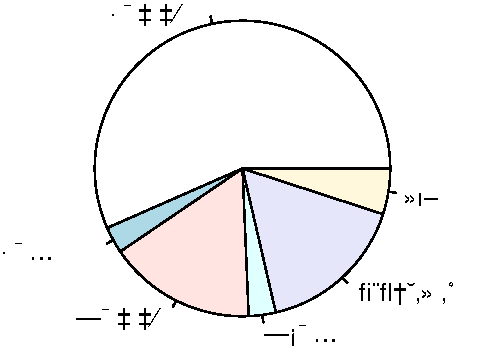
\includegraphics{linear_regression_files/figure-latex/unnamed-chunk-10-1.pdf}
当然建模的目的是需要考虑的,如果你是为了验证动态CAPM模型的效果,针对观测噪声项目的检验是必要的。比如,均值、独立性、正态性等。此处我们省略。

\end{document}
